% Critical Assessment and Selection of a Two-Phase CO2 Wellbore
% Blowdown Model -- HyperCO2 project research review.
%
% Source of record: docs/two_phase_model_assessment.md in
% github.com/JaderBarbosaLSU/hyperco2-wellbore (commit 752bd18).
% body.tex is the pandoc conversion of that document; edit body.tex
% for content, this file for layout. References are inline with DOIs
% and links; items the review could not verify against a primary
% source are marked [unverified] in the text.
\documentclass[11pt]{article}
\usepackage[margin=1in]{geometry}
\usepackage[round]{natbib}
% Unicode characters used literally by the pandoc-converted body.tex
\DeclareUnicodeCharacter{2080}{\ensuremath{_0}}
\DeclareUnicodeCharacter{2082}{\ensuremath{_2}}
\DeclareUnicodeCharacter{2084}{\ensuremath{_4}}
\DeclareUnicodeCharacter{2070}{\ensuremath{^0}}
\DeclareUnicodeCharacter{2074}{\ensuremath{^4}}
\DeclareUnicodeCharacter{2075}{\ensuremath{^5}}
\DeclareUnicodeCharacter{207B}{\ensuremath{^{-}}}
\DeclareUnicodeCharacter{0393}{\ensuremath{\Gamma}}
\DeclareUnicodeCharacter{0394}{\ensuremath{\Delta}}
\DeclareUnicodeCharacter{03B1}{\ensuremath{\alpha}}
\DeclareUnicodeCharacter{03B5}{\ensuremath{\varepsilon}}
\DeclareUnicodeCharacter{03B8}{\ensuremath{\theta}}
\DeclareUnicodeCharacter{03BC}{\ensuremath{\mu}}
\DeclareUnicodeCharacter{03C0}{\ensuremath{\pi}}
\DeclareUnicodeCharacter{03C1}{\ensuremath{\rho}}
\DeclareUnicodeCharacter{03C6}{\ensuremath{\varphi}}
\DeclareUnicodeCharacter{2016}{\ensuremath{\|}}
\DeclareUnicodeCharacter{2032}{\ensuremath{'}}
\DeclareUnicodeCharacter{2033}{\ensuremath{''}}
\DeclareUnicodeCharacter{2192}{\ensuremath{\rightarrow}}
\DeclareUnicodeCharacter{2194}{\ensuremath{\leftrightarrow}}
\DeclareUnicodeCharacter{2202}{\ensuremath{\partial}}
\DeclareUnicodeCharacter{2208}{\ensuremath{\in}}
\DeclareUnicodeCharacter{2212}{\ensuremath{-}}
\DeclareUnicodeCharacter{221D}{\ensuremath{\propto}}
\DeclareUnicodeCharacter{2248}{\ensuremath{\approx}}
\DeclareUnicodeCharacter{2264}{\ensuremath{\leq}}
\DeclareUnicodeCharacter{2265}{\ensuremath{\geq}}
\DeclareUnicodeCharacter{226A}{\ensuremath{\ll}}
\DeclareUnicodeCharacter{2272}{\ensuremath{\lesssim}}
\DeclareUnicodeCharacter{2273}{\ensuremath{\gtrsim}}
\usepackage{amsmath,amssymb,graphicx,booktabs,longtable,array,calc}
\usepackage{siunitx}
\usepackage{tikz}
\usetikzlibrary{arrows.meta,positioning,shapes.geometric}
\usepackage[colorlinks=true,linkcolor=blue,citecolor=blue,urlcolor=blue]{hyperref}
\usepackage{cleveref}
% pandoc compatibility macros used by body.tex
\providecommand{\tightlist}{\setlength{\itemsep}{0pt}\setlength{\parskip}{0pt}}
\providecommand{\pandocbounded}[1]{#1}
\newcommand{\real}[1]{#1}
\setcounter{secnumdepth}{0}   % headings carry their own numbers

\title{Two-Phase CO$_2$ Wellbore Blowdown Modeling and the\\
Closed-Loop Experimental Facility: Critical Assessment\\
and Conceptual Design}
\author{HyperCO2 project research review\\
\small Craft \& Hawkins Department of Petroleum Engineering, LSU ---
PERTT Lab}
\date{October 20, 2026}

\begin{document}
\maketitle

\begin{abstract}
\noindent Literature-supported assessment of two-phase modeling
approaches (HEM, HRM, drift-flux, two-fluid) for extending the
verified single-phase HyperCO2 wellbore blowdown solver to two-phase
liquid--vapor CO$_2$ flow. The Homogeneous Equilibrium Model is found
to be the defensible starting point on quantitative grounds, with
three bounded caveats: choke-discharge underprediction belongs at the
boundary, the equilibrium sound speed is discontinuous at the vapor
dome, and no-slip fails in the low-rate tail. The assessment covers
the governing formulation, the $(\rho,e)$ equilibrium flash with
Span--Wagner, transport closures, HLLC implications, a staged model
hierarchy, a verification/validation plan against named open
datasets, implications for fiber-optic DTS interpretation, and a
prioritized roadmap. Four publishable gaps are identified, all within
reach of the PERTT facility. Part~II is a preliminary engineering
feasibility study of the surface facility for repeated closed-loop
charging and discharging of the 2,000-ft well: operating scenarios,
five candidate configurations with computed Span--Wagner
thermodynamics, compressor-versus-pump analysis, storage and receiver
sizing, energy and turnaround estimates, instrumentation, safety, and
the coupling of lumped surface-equipment models to the transient
wellbore solver as a digital twin. The recommended configuration
anchors the loop on refrigerated liquid storage
(\SI{2.0}{MPa}/\SI{-20}{\celsius}) with pump--vaporizer charging, a
low-pressure buffer with condensing recovery, and a vented reference
mode --- rejecting both the single-gas-tank and compressor-charged
concepts on quantitative grounds.
\end{abstract}

\tableofcontents
\clearpage

\part*{Part I --- Critical Assessment and Selection of the Two-Phase
Model}
\addcontentsline{toc}{part}{Part I --- Two-phase model selection}

\hypertarget{hem-survives-scrutiny-as-the-starting-point}{%
\section{HEM Survives Scrutiny as the Starting
Point}\label{hem-survives-scrutiny-as-the-starting-point}}

\textbf{Bottom line: the Homogeneous Equilibrium Model is a defensible
--- indeed, the literature-optimal --- first extension of the existing
single-phase solver, but only with three explicit caveats attached.} The
quantitative case is strong: fitted CO₂ phase-change relaxation times
are \textbf{0.04--2.82 ms} against a wellbore blowdown time scale of
minutes (equilibrium Damköhler number ≳10⁵), the only controlled
vertical two-phase CO₂ dataset found near-zero slip at 6.5 MPa, and
SINTEF's own six-equation two-fluid model ``did not clearly outperform
the HEM'' against pipe-depressurization data. The caveats: (i) HEM
systematically underpredicts choked discharge through short restrictions
by 0--26\% --- which is why the choke boundary, not the wellbore
interior, should carry the non-equilibrium correction; (ii) the HEM
mixture sound speed is discontinuous at the saturation boundary, the
principal numerical hazard for the HLLC solver; and (iii) the no-slip
assumption fails precisely in the late-blowdown, low-rate tail, where
condensate fallback in a 17 cm bore at an area ratio of
\textasciitilde200:1 to the 12.7 mm choke is governed by drift
velocities of order 0.1--1 m/s that exceed the mixture velocity. The
staged path HEM → HRM → drift-flux is mathematically protected by the
subcharacteristic condition (each added equilibrium assumption lowers
the sound speed, so the equilibrium limit is a well-behaved limit of the
relaxation system), and the whole architecture --- MUSCL-Hancock/HLLC,
Span--Wagner tabulated closure, conjugate radial heat transfer,
quasi-steady choke boundary --- survives the extension essentially
intact. The deepest finding of this review is negative and valuable:
\textbf{no vertical CO₂ blowdown dataset, no published CO₂-well DTS
phase-transition trace, no measured condensation-side relaxation time,
and no transport closure validated above \textasciitilde10 mm diameter
exist} --- four publishable gaps the planned PERTT experiment sits
directly on.

\begin{center}\rule{0.5\linewidth}{0.5pt}\end{center}

\hypertarget{the-literature-splits-into-pipeline-decompression-choke-discharge-and-a-thin-wellbore-corpus}{%
\subsection{1. The literature splits into pipeline decompression, choke
discharge, and a thin wellbore
corpus}\label{the-literature-splits-into-pipeline-decompression-choke-discharge-and-a-thin-wellbore-corpus}}

The transient CO₂ depressurization literature has three centers of
gravity --- SINTEF/NTNU (pipe depressurization, relaxation-model theory,
choked orifice flow), UCL/Mahgerefteh (pipeline rupture, HRM, solids)
--- and a smaller wellbore corpus (LBNL/T2Well, SINTEF well models,
OLGA). The per-study record below carries forward the research notes'
verification flags: references marked \textbf{{[}unverified{]}} were not
confirmed against a primary source and must be checked before citation.

\hypertarget{pipeline-and-shock-tube-decompression}{%
\subsubsection{1.1 Pipeline and shock-tube
decompression}\label{pipeline-and-shock-tube-decompression}}

\textbf{\citet{munkejord2020} --- the anchor dataset.} ECCSEL rig: 61.67 m
SS316 horizontal tube, 40.8 mm ID, honed bore, 16 Kulite transducers
logged at 100 kHz concentrated near the rupture end, 23 Type-E
thermocouples (±0.22 °C) including top/side/bottom triplets at four
stations, full-bore rupture-disc opening; pressure uncertainty 60 kPa
(95\%). Tests span gas-phase (Test 3: \textbf{4.04 MPa, 10.2 °C} --- the
closest published analog to the 2,000-ft well's initial state) to dense
phase (12.54 MPa/21.1 °C; 10.40 MPa/40 °C), plus an N₂ single-phase
reference. Model: HEM with Span--Wagner EOS. Conclusions: single-phase
wave speeds match Span--Wagner ``very well''; measured two-phase plateau
pressures fall \textbf{below} the equilibrium prediction (delayed
flashing); the equilibrium wave-speed kink (e.g., \textasciitilde370 m/s
→ \textless40 m/s at the phase boundary in Test 8) is measured as a
smooth transition lying between equilibrium and frozen curves; HEM
predicts dry-out \textasciitilde0.5 s early; in the gas-phase Test 3,
condensation droplets appear near \textbf{2.8 MPa, below the equilibrium
dew pressure} --- delayed condensation, the gas-side analog of delayed
flashing; the N₂ closed-end comparison exposed a
heat-transfer-correlation failure at low velocity (−150 °C predicted vs
−78 °C measured), not a phase-equilibrium failure. Raw data are open \citep{sintef2020data} (\href{https://www.pvv.ntnu.no/~stm/dring/depress-co2-exp.pdf}{preprint};
\href{https://sintef.brage.unit.no/sintef-xmlui/handle/11250/2770324}{SINTEF
Brage}).

\textbf{\citet{munkejord2021}} --- same rig, CO₂--N₂ and CO₂--He;
isoenergetic--isochoric flash via an in-house VLE algorithm interfaced
to TREND; decompression-wave speed ``abruptly decreases from about 350
m/s to 40 m/s at 6 MPa'' under full equilibrium; the production numerics
are the dissipative FORCE flux + MUSCL + SSP-RK2 at CFL 0.85, 1200--4800
cells; open data \citep{sintef2021data} (\href{https://www.pvv.ntnu.no/~stm/dring/depress-mix-exp.pdf}{preprint}).

\textbf{\citet{log2024hrm}} --- HEM vs HRM* (constant,
per-case-fitted relaxation time) across initial temperatures 10--40 °C:
the fitted relaxation time \textbf{decreases with initial temperature
and spans \textasciitilde60×}, 0.04 ms (40 °C) / 1.50 ms (21 °C) / 2.82
ms (4.6 °C)
(\href{https://sintef.brage.unit.no/sintef-xmlui/handle/11250/3103647}{Brage
record}).

\textbf{\citet{log2024hfm} (HFM)}
--- a four-equation homogeneous model plus
bubble-number/interfacial-area transport, CNT homogeneous nucleation
plus fitted heterogeneous rates (``not predictive''), kinetic-theory
evaporation; one global parameter set achieves MAPE \textbf{6.0\% vs
7.6\%} for per-case-tuned HRM*; numerics are Godunov splitting + HLLC +
implicit Euler sources. Metastability findings: near-critical dome
entries (1.2 K below T\_c) show essentially zero undershoot; five colder
tests flashed where CNT predicts \textless10⁻¹⁰ bubbles m⁻³s⁻¹,
implicating un-modeled heterogeneous nucleation; crack-tip pressures
reach 20\% below saturation
(\href{https://www.pvv.ntnu.no/~stm/dring/hfm_preprint.pdf}{HFM
preprint}).

\textbf{\citet{munkejord2015}} --- HEM vs a six-equation two-fluid model
(both thermodynamic-equilibrium; slip via interfacial + wall friction),
Peng--Robinson + TRAPP transport, validated on National Grid Test 31
\citep{cosham2012}, Botros CO₂--CH₄, Drescher CO₂--N₂. Dry-out timing
errors of opposite sign (HEM \textasciitilde2 s early, TFM
\textasciitilde4 s late on the 90\% CO₂ case); the authors conclude the
TFM \textbf{``did not clearly outperform the HEM''} and prefer HEM for
simplicity, noting better TFM closures would require local experimental
data that do not exist
(\href{https://www.sintef.no/globalassets/project/co2-dynamics/publications/depress-mix-preprint.pdf}{preprint}).

\textbf{\citet{brown2013}} --- HRM for full-bore rupture of
dense-phase CO₂ pipelines with an empirically derived relaxation-time
equation; verified on hypothetical shock tubes, validated against
CO2PipeHaz full-bore ruptures. The load-bearing conclusion:
\textbf{delayed phase transition has negligible effect on the
decompression-wave rate, but ignoring it underestimates the transient
discharge rate}
(\href{https://www.scipedia.com/public/Brown_et_al_2013a}{Scipedia};
\href{https://hal-ineris.archives-ouvertes.fr/ineris-00963485}{HAL-INERIS}).
The exact relaxation-time correlation and EOS were not retrievable from
open pages \textbf{{[}Downar-Zapolski-form refit + Peng--Robinson
recalled from training, unverified{]}}.

\textbf{\citet{martynov2018}} --- 36.7 m, 50 mm pipe, ≤45 bar, 4/6 mm
orifices: pressure and temperature stabilize near the triple point;
video shows liquid/vapour \textbf{stratification then rapid solid-CO₂
formation}; an HEM-based model with vapor--liquid--solid properties
predicts P(t), T(t) and solid mass, self-described as ``partially
validated''
(\href{https://eprints.whiterose.ac.uk/id/eprint/130497}{White Rose}).
The observed stratification before solidification is direct evidence
that homogeneous assumptions degrade near the triple point.

\textbf{Botros et al.~shock tubes} (decompression-wave speed vs
pressure, the fracture-control community's standard): \citet{botros2010}; \textbf{\citet{botros2016} (the key pure-CO₂ paper)}; plus
binary-impurity companions in JPVT 139(2) (DOI 10.1115/1.4034016,
10.1115/1.4034466) and \emph{Can. J. Chem. Eng.} 95(3):440--448 (DOI
10.1002/cjce.22689) --- all DOIs verified from the reference list of \citet{munkejord2021}
(\href{https://www.pvv.ntnu.no/~stm/dring/depress-mix-exp.pdf}{mirror}).
Rig dimensions (\textasciitilde42 m, \textasciitilde38 mm ID) are
\textbf{{[}unverified{]}}.

\textbf{COOLTRANS (National Grid/Spadeadam)} --- \citet{cosham2012}: 144 m × 150 mm shock tube; pressure ``fell to saturation quickly, with
little variation along the 144 m length.'' The vertical venting rig
(dense CO₂ at 150 barg through 12/25/50 mm vertical vents, Coriolis mass
flow) found predictions matching the smaller vents while the \textbf{50
mm vent out-flowed homogeneous-equilibrium predictions --- delayed
nucleation}; small amounts of solid CO₂ were observed in vents and
craters
(\href{https://www.icheme.org/media/9161/paper20-hazards-23.pdf}{Allason
et al., Hazards XXIII}).

\textbf{Guo et al.~(DUT/UCL, CO2QUEST)} --- 258 m × 233 mm
industrial-scale pipeline discharging through a \textbf{vertical 15 mm
orifice}; Test 1 is \textbf{gaseous CO₂ at 3.7 MPa, 37.5 °C} --- the
single large-scale test closest to the well's initial state, including
the vertical exit geometry; 10 pressure sensors at 100 kHz, 24
thermocouples resolving top/bottom stratification
(\href{https://discovery-pp.ucl.ac.uk/id/eprint/10051724/1/Manuscript_01.pdf}{UCL
manuscript}). Companion journal papers (Applied Energy 178:189--197;
Applied Energy 183:1279--1291; Energy 119:53--66) are cited from that
manuscript's reference list without DOIs.

\textbf{Vessel blowdowns}: \citet{gebbeken1996} supercritical-CO₂ vessel blowdown with void fraction and stratification is the classical reference but its full citation \textbf{could not be verified this session {[}unverified --- training recollection{]}}. A 2025 open dataset exists for a 2 m³ sphere to
130 bar and −50 °C (INERIS;
\href{https://www.ncbi.nlm.nih.gov/pmc/articles/PMC12819109/}{PMC12819109},
title and PMC ID only --- retrieve before use).

\hypertarget{chokeorifice-critical-flow}{%
\subsubsection{1.2 Choke/orifice critical
flow}\label{chokeorifice-critical-flow}}

\textbf{\citet{hammer2022} --- the direct precedent for the planned architecture.} Six
pipe blowdowns from \textasciitilde12 MPa/25 °C through orifices and
nozzles of 4.5, 9.0 and \textbf{12.7 mm} (the exact target choke size),
coupled to a 1-D transient HEM pipe solver (4800 cells, MUSCL+RK,
Friedel friction). Findings: \textbf{``the choke point is at a
non-equilibrium state''}; HEM mass-flux error −26\% to 0\% (always
underpredicting), Henry--Fauske −22\% to +5\%, delayed-HEM (flashing
deferred to the CNT superheat limit) −21\% to +10\%; against
Banasiak--Hafner nozzle data, MARE 7.8\% (HEM), 2.5\% (D-HEM), 5.4\%
(HF), with HEM degrading to 17\% on the low-pressure subset. Orifice
contraction coefficients computed from a Bragg-type force balance:
\textbf{C\_c = 0.75 (12.7 mm), 0.74 (9.0 and 4.5 mm)}, from the
incompressible sharp-edge limit π/(π+2) ≈ 0.611; the authors state the
orifice value remains uncertain. HEM's choke search ``often'' locks at
the saturation crossing because the sound speed is discontinuous there
(\href{https://sintef.brage.unit.no/sintef-xmlui/handle/11250/3023978}{SINTEF
record};
\href{https://www.pvv.ntnu.no/~stm/dring/outflow_preprint.pdf}{preprint}).

\textbf{Boccardi et al.~(ENEA)} --- 107 steam-water PSV tests (6 mm
orifice, 0.5--1.75 MPa, inlet quality 0.5--10\%): HEM never
overestimated, underpredicting 2--40\%; HNE-DS variance 6.9\%;
Henry--Fauske mean −0.25\% but overestimating up to 27.4\%
(\href{https://www.aidic.it/CISAP4/webpapers/33Boccardi.pdf}{CISAP4
paper}). Fauske's relaxation-length framework (non-equilibrium vanishes
beyond \textasciitilde0.1 m flow length) is documented in a LANL review
(\href{https://public.lanl.gov/davidp/MSThesisHTML/2.html}{LANL thesis
review}). \citet{henry1971} and the N = x\_eq/0.14 form are \textbf{{[}unverified --- check
original{]}}; \citet{morris1990} reports
±6--7\% reproduction of choked gas-liquid flow by empirical C\_d
correlations
(\href{https://researchportal.hw.ac.uk/en/publications/discharge-coefficients-for-choked-gas-liquid-flow-through-nozzles/}{portal}).

\hypertarget{wellbore-flow}{%
\subsubsection{1.3 Wellbore flow}\label{wellbore-flow}}

\textbf{T2Well/ECO2N \citep{pan2011}} --- 1-D
transient non-isothermal \textbf{drift-flux} CO₂--water--NaCl wellbore
model coupled to TOUGH2/ECO2N: fully implicit mass/energy (Newton),
semi-explicit mixture momentum; \citet{shi2005} slip closure with
profile parameter C₀ capped 1.0--1.5 and a Kutateladze-number drift
velocity re-tuned to Ku = 142 (vs Richter's 75); Ramey or gridded radial
heat exchange; explicitly \textbf{cannot represent coexisting liquid +
gaseous CO₂ with a third phase}; drift velocities 0.28--0.72 m/s in its
verification case; validation limited to analytics and leakage scenarios
--- no field two-phase data
(\href{https://escholarship.org/content/qt0k35m2vg/qt0k35m2vg.pdf}{manual
PDF}; \href{https://www.osti.gov/biblio/1007233}{OSTI 1007233}). \citet{shi2005} itself was obtained only second-hand
\textbf{{[}forms must be taken from the original{]}}.

\textbf{SINTEF two-fluid well model \citep{linga2016}} --- two-fluid vertical-well model with
conjugate conduction through tubing/annulus/casing/cement/rock; phase
mass transfer via \textbf{relaxation source terms that satisfy the
second law and are continuous in the single-phase limit} (engineered
specifically for a robust single↔two-phase transition);
flow-regime-dependent friction and heat transfer; Span--Wagner EOS;
applied to shut-in and blowout
(\href{https://sintef.brage.unit.no/sintef-xmlui/handle/11250/2620521}{Brage
record}; author attribution to Linga \& Lund \textbf{unverified}).

\textbf{UCL well model (Samuel \& Mahgerefteh)} --- 1-D HEM,
conservative hyperbolic form, Godunov FV, Peng--Robinson EOS, Chen
friction, Dittus--Boelter in-well heat transfer, wellhead ghost cells
with isentropic/Thompson characteristic relations; \textbf{validated
against Ketzin single-phase wellbore temperatures} (0.41 kg/s; Möller et
al.~2014 data) and benchmarked against OLGA, where PR gave
systematically lower temperatures --- a cubic-EOS bias argument for
Span--Wagner
(\href{https://discovery-pp.ucl.ac.uk/10080131/3/Samuel\%20Ramp-up\%20injection\%20paper.pdf}{UCL
PDF}). Their Goldeneye ramp-up cases show slower ramps giving
\emph{colder} wellhead minima (252/238/226 K for 5 min/30 min/2 h
ramps).

\textbf{\citet{lindeberg2011} (SINTEF, TCCS-6)} --- quasi-steady marching
blowout model of the Sleipner well: rates 181--313 kg/s, outlet
temperatures −75 to −97 °C, hydrate zones 200--550 m below wellhead with
plug-melt \textbf{pulsed release}; dry ice in the well judged unlikely;
explicitly called for an instrumented abandoned-well blowout experiment
(\href{https://www.sintef.no/globalassets/project/tccs6/presentations/e6/03_co2blowout.pdf}{TCCS-6
PDF}). His adiabatic-well conclusion applies to sustained high-rate
blowouts and \textbf{does not transfer} to a slow, finite-inventory,
choked blowdown where conjugate wall heat input is first-order.

\textbf{\citet{hammer2021} (preprint; journal of record unconfirmed)} --- the only controlled vertical
two-phase CO₂ dataset: IFE FALCON loop, \textbf{44 mm vertical pipe at
6.5 MPa}, superficial velocities 0.2--4.0 m/s (gas) / 0.15--3.0 m/s
(liquid), holdup by X-ray and gamma densitometry. Result: \textbf{``the
experiments show nearly no-slip flow, except at low inlet liquid
holdup,'' and ``the simplest model, the homogeneous no-slip approach,
performed best''} --- beating both \citet{shi2005} and the T2Well adaptation, because gas and liquid properties converge near the critical
point
(\href{https://www.pvv.ntnu.no/~stm/dring/driftflux-well.pdf}{preprint}).

\textbf{Field/industry context}: \citet{wildwell2024} (Havtil note 2024-380) documents dry ice ejected from wellbores, frozen annuli at
\textasciitilde100 m casing shoes, and the judgment that with CO₂'s
critical point inside typical operating envelopes ``a phase change is
almost guaranteed somewhere in the wellbore if control is lost''; the
new OLGA CO₂ solver tightens p--T coupling for stability but is
proprietary
(\href{https://www.havtil.no/contentassets/9b77c8de198b49afb887f9688b45f4be/havtil_co2-blowoutconsiderations_techncialnote_2024-380.pdf}{Havtil
PDF}).

\textbf{Negative results carried forward explicitly}: no measured
in-well dataset from any CO₂ well blowdown exists in the open
literature; no DTS record of a two-phase CO₂ column tracking T\_sat(p)
was found (Ketzin deliberately avoided two-phase operation with N₂
flushes, keeping \textasciitilde3 °C margin to the condensation line ---
\href{https://iahs.info/uploads/dms/15943.50-286-290-355-40-Wiese.pdf}{Wiese
et al.~2012};
\href{https://gfzpublic.gfz-potsdam.de/pubman/item/item_242409_1/component/file_242408/15975.pdf}{Würdemann
et al.~2010}); no CO₂-specific CCFL/flooding study for vertical
wellbores was found; Ruan et al.~(IJGGC 2013) and Lu \& Connell wellbore
papers \textbf{could not be located --- do not cite}.

\hypertarget{model-comparison-the-relaxation-hierarchy-orders-the-choices-and-the-data-refuse-to-reward-complexity}{%
\subsection{2. Model comparison: the relaxation hierarchy orders the
choices and the data refuse to reward
complexity}\label{model-comparison-the-relaxation-hierarchy-orders-the-choices-and-the-data-refuse-to-reward-complexity}}

The mathematically clean frame is the relaxation hierarchy of \citet{lund2012} (\href{https://www.sintef.no/globalassets/project/co2-dynamics/publications/lund_two-phase_relaxation_hierarchy.pdf}{SINTEF PDF}; journal metadata \textbf{{[}from training, unverified{]}}): a homogeneous
(single-velocity) two-phase model with three relaxation processes ---
volume transfer driven by Δp, heat by ΔT, mass by Δμ --- generates eight
models; imposing each equilibrium \textbf{lowers} the mixture sound
speed through sum-of-squares increments (1/ã²\_X = 1/ã²\_Y + Z ≥ 0), so
every equilibrium limit satisfies the \textbf{subcharacteristic
condition} for any thermodynamically stable EOS. HEM (p--T--μ
equilibrium) is the bottom of the hierarchy with the lowest sound speed
and is the \textbf{only} member whose sound speed is discontinuous at
the single-phase boundary. HRM is the hierarchy's pT model with finite
μ-relaxation --- strictly dissipative relative to HEM and smooth at the
dome boundary. Velocity non-equilibrium (drift-flux, two-fluid) sits
outside the proven ordering; Lund defers it explicitly.

Against this frame, the empirical record is one-directional. HEM with a
reference EOS captures decompression-wave speeds well and bulk two-phase
behavior ``fairly'' but overpredicts the pressure plateau for dense
initial states and underpredicts short-restriction discharge; HRM* fixes
the plateau at the cost of a case-dependent relaxation time (0.04--2.82
ms, \textasciitilde60× spread); the nucleation-based HFM achieves
HRM*-level accuracy (MAPE 6.0\% vs 7.6\%) with one global parameter set
but fitted heterogeneous rates; the six-equation two-fluid model did
\textbf{not} beat HEM and its own authors recommend HEM
(\citealp{munkejord2015}, \href{https://www.sintef.no/globalassets/project/co2-dynamics/publications/depress-mix-preprint.pdf}{preprint}; \citealp{log2024hfm}, \href{https://www.pvv.ntnu.no/~stm/dring/hfm_preprint.pdf}{HFM preprint}). Drift-flux earns its keep only where mixture velocity falls
to the drift-velocity scale --- O(0.1--1 m/s) per T2Well's Kutateladze
closure --- and the one vertical CO₂ dataset shows no-slip winning
outright at 6.5 MPa
(\citealp{hammer2021}, \href{https://www.pvv.ntnu.no/~stm/dring/driftflux-well.pdf}{preprint}). No Saurel-type seven-equation CO₂ decompression
validation was located; conditional hyperbolicity of single-pressure
six-equation models and the Baer--Nunziato remedy are standard knowledge
\textbf{{[}unverified primary{]}}.

\begin{longtable}[]{@{}
  >{\raggedright\arraybackslash}p{(\columnwidth - 10\tabcolsep) * \real{0.1667}}
  >{\raggedright\arraybackslash}p{(\columnwidth - 10\tabcolsep) * \real{0.1667}}
  >{\raggedright\arraybackslash}p{(\columnwidth - 10\tabcolsep) * \real{0.1667}}
  >{\raggedright\arraybackslash}p{(\columnwidth - 10\tabcolsep) * \real{0.1667}}
  >{\raggedright\arraybackslash}p{(\columnwidth - 10\tabcolsep) * \real{0.1667}}
  >{\raggedright\arraybackslash}p{(\columnwidth - 10\tabcolsep) * \real{0.1667}}@{}}
\toprule\noalign{}
\begin{minipage}[b]{\linewidth}\raggedright
Criterion
\end{minipage} & \begin{minipage}[b]{\linewidth}\raggedright
HEM (3 eq.)
\end{minipage} & \begin{minipage}[b]{\linewidth}\raggedright
HRM/HRM* (4 eq.)
\end{minipage} & \begin{minipage}[b]{\linewidth}\raggedright
HFM (4 eq. + nucleation)
\end{minipage} & \begin{minipage}[b]{\linewidth}\raggedright
Drift-flux (3--4 eq. + slip law)
\end{minipage} & \begin{minipage}[b]{\linewidth}\raggedright
Two-fluid (6--7 eq.)
\end{minipage} \\
\midrule\noalign{}
\endhead
\bottomrule\noalign{}
\endlastfoot
PDEs added to current solver & 0 & +1 (vapor mass) & +2--3 (bubble
number/area) & 0--1 (algebraic slip in fluxes) & +3--4 \\
Closures beyond EOS & none & relaxation time θ & nucleation rates,
growth law & C₀(α), v\_drift (\citealp{shi2005}/T2Well) & interfacial friction,
Δp regularization, per-phase wall laws \\
Closure uncertainty for CO₂ & none (by construction) & θ spans 0.04--2.8
ms, \textasciitilde60×; \textbf{condensation-side θ uncharacterized} &
heterogeneous rates ``not predictive'' & untested for CO₂ at low rates;
no-slip beat it at 6.5 MPa & ``would require local data that do not
exist'' (SINTEF) \\
Documented CO₂ fidelity & wave speeds good; plateau over-, discharge
under-predicted (0--26\% at chokes) & plateau corrected; MAPE 7.6\% &
MAPE 6.0\%, one parameter set & mispredicted FALCON holdup; needed for
fallback regime & did not clearly outperform HEM \\
Numerical robustness & sound-speed discontinuity at dome; otherwise
hyperbolic, conservative & smooth (frozen) acoustics --- \emph{better}
than HEM & stiff sources (implicit Euler) & preserves conservative
structure & conditional hyperbolicity (6-eq.); \textasciitilde2× state
size (7-eq.) \\
Relative cost & 1 (flash-dominated) & \textasciitilde1.1 &
\textasciitilde1.3--1.5 & \textasciitilde1.05 & ≥2 \\
Validation data available & SINTEF/Botros/COOLTRANS/Guo & same (plateau
level) & same & FALCON loop only (44 mm, 6.5 MPa) & none that
discriminates \\
\end{longtable}

\hypertarget{verdict-hem-is-defensible-as-the-starting-point-with-the-failure-modes-named-and-bounded}{%
\subsection{3. Verdict: HEM is defensible as the starting point --- with
the failure modes named and
bounded}\label{verdict-hem-is-defensible-as-the-starting-point-with-the-failure-modes-named-and-bounded}}

The working hypothesis survives critical testing on every quantitative
axis examined, provided its documented biases are treated as known
model-form error rather than discovered later.

\textbf{Time scales.} Fitted CO₂ flashing relaxation times are
0.04--2.82 ms (\citealp{log2024hrm}, \href{https://www.pvv.ntnu.no/~stm/dring/hfm_preprint.pdf}{HFM preprint}); the well drains through a 12.7 mm choke over minutes. Taking
θ ≤ 3 ms against a transport residence time of 10¹--10² s (mixture
velocities of order 1--10 m/s over 610 m), the equilibrium Damköhler
number is ≥10⁴--10⁵: local equilibrium is an excellent bulk
approximation everywhere except within the first metres behind a fast
rarefaction head and inside the choke itself (transit ≤
\textasciitilde0.25 ms at 50--100 m/s through a plate ≤ one diameter
thick --- firmly inside Fauske's \textasciitilde0.1 m non-equilibrium
regime, \href{https://public.lanl.gov/davidp/MSThesisHTML/2.html}{LANL
review}).

\textbf{Metastability.} The documented HEM plateau errors are for
dense/liquid inventories. For a gas-phase start, the relevant
non-equilibrium is delayed condensation --- observed once (droplets at
2.8 MPa vs higher equilibrium dew pressure, Test 3, \citealp{munkejord2020}, \href{https://www.pvv.ntnu.no/~stm/dring/depress-co2-exp.pdf}{preprint}) and bounded by CNT in \citet{hammer2025}. Near-critical dome entries show essentially zero
undershoot, and the well starts at reduced temperature ≈ 0.99--1.06, so
the warm early inventory crosses the dome nearly in equilibrium;
supercooling grows as the column cools. Crucially, \textbf{no measured
condensation-side relaxation time exists} --- the 0.04--2.8 ms values
are all flashing-side. This is simultaneously the weakest link in the
HEM justification and a publishable gap.

\textbf{Slip.} At 6.5 MPa in a 44 mm vertical pipe, no-slip beat every
drift-flux law tested
(\citealp{hammer2021}, \href{https://www.pvv.ntnu.no/~stm/dring/driftflux-well.pdf}{preprint}) --- but their own caveat, ``except at low inlet liquid
holdup,'' flags the regime where the blowdown problem lives. At 1--4 MPa
the liquid/vapor density ratio reaches order 10--50; the choked mass
flux through 12.7 mm, spread over a bore with \textasciitilde200× the
area, gives in-bore superficial velocities that fall to and below the
O(0.3--0.7 m/s) Kutateladze drift velocity. Below the Turner-type
critical gas velocity, condensate cannot be lifted: fallback, a liquid
sump on the closed bottom, and countercurrent segregation follow --- and
HEM then mispredicts inventory distribution and the DTS-visible
phase-front locations. This is an inference from cited density/geometry
facts plus standard flooding physics; no CO₂-well demonstration exists.

\textbf{Known mispredictions to expect.} Wave propagation: equilibrium
kink too sharp; measured transition smooth, between equilibrium and
frozen curves. Quality/dry-out: \textasciitilde0.5--2 s early in 61.7 m
pipes. Temperature: tracks T\_sat(p) correctly while two-phase (the
saturation clamp is HEM's most reliable output); the large temperature
errors observed are heat-transfer-closure failures, not equilibrium
failures. Discharge: 0--26\% underprediction at short restrictions,
which couples back into the pressure history (HEM at the choke
overpredicted the pipe plateau in \citealp{hammer2022}).

\textbf{Transitions and limits.} The single↔two-phase transition is
thermodynamically trivial in HEM (the flash decides) but numerically
delicate (Section 9). Near-critical: the lever rule degenerates and the
flash ill-conditions as ρ′−ρ″→0; published codes handle it by dense
tabulation, nothing smarter was found. Triple point (0.518 MPa, 216.59
K): reachable only late and essentially at/downstream of the choke; the
pure-CO₂ equilibrium sound speed is \textbf{zero at the triple point}
(\citealp{munkejord2021}, \href{https://www.pvv.ntnu.no/~stm/dring/depress-mix-exp.pdf}{preprint}), so the wellbore model should not carry a solid phase
--- a three-phase flash belongs in the choke submodel if at all (\citealp{hammer2013} provides the thermodynamic machinery).

\textbf{Global vs local reliability --- the honest summary.} HEM is
trustworthy for globally conserved and saturation-clamped quantities:
pressure histories, inventory, two-phase column temperature, wave
arrival to within the smoothing noted. It is untrustworthy for local,
closure-sensitive quantities: discharge rate through short restrictions,
local quality/void during fast transients, dry-out timing, phase
distribution at low rates, and anything downstream of the triple point.
The staged plan should be read as: Stage 1 earns the global quantities;
the later stages chase the local ones.

\hypertarget{hem-governing-equations-the-solver-changes-less-than-the-closures-do}{%
\subsection{4. HEM governing equations: the solver changes less than the
closures
do}\label{hem-governing-equations-the-solver-changes-less-than-the-closures-do}}

In conservative mixture form, with mixture density ρ, velocity u, total
energy E = ρ(e + u²/2), well inclination giving gravity component g\_z,
area A constant:

\[\frac{\partial \rho}{\partial t} + \frac{\partial (\rho u)}{\partial x} = 0\]

\[\frac{\partial (\rho u)}{\partial t} + \frac{\partial (\rho u^2 + p)}{\partial x} = -\rho g_z - \frac{f_D}{2D}\rho u |u|\]

\[\frac{\partial E}{\partial t} + \frac{\partial\big[(E + p)u\big]}{\partial x} = -\rho g_z u + \frac{4 q''_w}{D}\]

These are \emph{identical in form} to the existing single-phase system.
Under full equilibrium, ρ and e are mixture quantities built from
saturated phase states at a common (p, T\_sat(p)):

\[\frac{1}{\rho} = v = (1-x)\,v'(T) + x\,v''(T), \qquad e = (1-x)\,e'(T) + x\,e''(T),\]

with quality x the lever-rule coordinate. Unchanged: the finite-volume
update, MUSCL-Hancock reconstruction (reconstruct in primitive variables
(ρ, u, p) as now), the conjugate completion/formation radial network and
its coupling through q″\_w, the gravity and geometry treatment, and the
fiber-optic output machinery. Changed: (i) the thermodynamic closure
(ρ,e)→(p,T,a) must return two-phase states, quality, and the
\textbf{equilibrium} sound speed a\_eq inside the dome (Section 5); (ii)
the friction closure needs a two-phase evaluation (Section 7); (iii) the
wall heat-transfer coefficient needs regime logic (Section 8); (iv) the
choke boundary needs a two-phase critical-flux routine and, per the
evidence, a non-equilibrium correction (Section 10). No new PDE, no new
wave family: eigenvalues remain u, u ± a with a = a\_eq(ρ,e) in the
dome. The full-equilibrium sound speed is (Flåtten \& Lund,
\href{https://www.sintef.no/globalassets/project/co2-dynamics/publications/subchar.pdf}{subchar.pdf}):

\[\frac{1}{a_{\mathrm{HEM}}^2} = \frac{1}{a_p^2} + \rho T\!\left[\frac{\rho_g \alpha_g}{c_{p,g}}\left(\frac{ds_g}{dp}\right)_{\!\mathrm{sat}}^2 + \frac{\rho_l \alpha_l}{c_{p,l}}\left(\frac{ds_l}{dp}\right)_{\!\mathrm{sat}}^2\right], \qquad \frac{1}{a_p^2} = \rho\left(\frac{\alpha_g}{\rho_g c_g^2} + \frac{\alpha_l}{\rho_l c_l^2}\right),\]

where a\_p is the Wood (mechanical-equilibrium) speed and the
saturation-line entropy derivatives supply the extra compliance from
phase change. Note a\_HEM ≤ a\_Wood ≤ a\_frozen --- the practical
consequence is that the explicit CFL constraint inside the dome is
\emph{looser} than in single phase; the time step stays governed by the
single-phase region.

\hypertarget{thermodynamic-closure-the-ux3c1e-flash-reduces-to-one-scalar-equation-in-t}{%
\subsection{5. Thermodynamic closure: the (ρ,e) flash reduces to one
scalar equation in
T}\label{thermodynamic-closure-the-ux3c1e-flash-reduces-to-one-scalar-equation-in-t}}

The published pattern (\citealp{giljarhus2012}, the foundational density--energy Span--Wagner method for CO₂ CFD; extended to vapor--liquid--solid in \citealp{hammer2013} ---
\href{https://pvv.ntnu.no/~stm/dring/publ.html}{Munkejord publ. list})
maps directly onto the existing code:

\textbf{Two-phase detection.} Given a cell's (ρ, e): compute the
saturated bracket energies e′\_sat(ρ), e″\_sat(ρ) from a precomputed 1-D
saturation-line table (T\_sat, p\_sat, ρ′, ρ″, e′, e″, s′, s″
parameterized by T). If e lies between the brackets (and ρ between
ρ″(T\_tr) and ρ′ limits), the state is in the dome; otherwise the
existing single-phase (ρ,e)→T Newton applies unchanged.

\textbf{The reduced flash.} For a pure substance, the general UV-flash
is 4 nonlinear equations, but saturation relations collapse it to
\textbf{one scalar equation in T}
(\citealp{kumar2024}, \href{https://arxiv.org/html/2408.09164v2}{arXiv:2408.09164}): with v = 1/ρ fixed,

\[F(T) = \big(1 - x(T)\big)\,e'(T) + x(T)\,e''(T) - e = 0, \qquad x(T) = \frac{v - v'(T)}{v''(T) - v'(T)},\]

solved by Newton with bisection safeguard inside the bracket; then p =
p\_sat(T), and a = a\_eq from the formula above (or the equivalent
(∂p/∂ρ)\_s with equilibrium-constrained derivatives, as SINTEF does).
\citet{kumar2024} report an order-of-magnitude CPU reduction on a tank
blowdown and 3--4× on an HLLC pipe case from this reduction alone. The
lever rule applies on v and e simultaneously by construction;
\textbf{quality x (mass fraction) and void fraction α = x v″/v must
never be conflated} --- α is what gravity head and DTS-visible density
respond to, x is what the energy balance transports; at 2 MPa, x = 0.1
corresponds to α ≈ 0.7--0.8.

\textbf{Acceleration.} Direct Span--Wagner evaluation can consume
\textasciitilde90\% of runtime; SINTEF's (T,p)-indexed look-up tables
achieved \textbf{100--300× speedups at \textasciitilde10⁻³ \% deviation}
(\href{https://www.sintef.no/en/publications/publication/1274087}{SINTEF
2007 record}). For the dome, the existing 512² (ln ρ, T) tables are
\emph{not} usable, since (ρ,T) is not a complete state pair under
saturation. Two published options: (a) \textbf{separate 1-D
saturation-line splines + reduced flash} --- the minimal change,
recommended; (b) a full (ρ,e)-space 2-D table spanning the dome ---
Brown et al.~(UCL) built adaptive inverse-interpolation tables on a
(ρ,U) grid with \textbf{70\% of nodes inside the envelope, 15\% each
hugging the dew and bubble lines}, Akima splines, mean deviations
0.005\% (T) and 0.44\% (p); a uniform (p,T) grid ``failed outright''
(\href{https://discovery.ucl.ac.uk/1522588/1/Brown\%20et\%20al\%20Thermodynamic\%20interpolation\%20for\%20the\%20simulation\%20of\%20two-phase\%20flow\%20of\%20non-ideal\%20mixtures\%20AAM.pdf}{UCL
Discovery PDF}). A rumored standalone ``SINTEF SW-spline'' journal paper
\textbf{does not verifiably exist} --- do not cite one.

\textbf{Near-critical behavior.} The lever rule degenerates as ρ′−ρ″ → 0
and the saturation-line Newton ill-conditions; no published special fix
was found beyond dense tabulation near T\_c --- flag this as an
implementation risk to be handled by local grid refinement of the
saturation table and a fallback to the single-phase branch within a
small ε of T\_c.

\textbf{CoolProp organization (background orientation, not from the
research notes --- standard knowledge, verify against CoolProp
documentation before citing):} CoolProp implements the Span--Wagner
Helmholtz formulation with (ρ,T) as native variables, uses ancillary
saturation equations as initial guesses for a Newton saturation solve,
routes general two-property flashes (including (ρ,e)\ldots{} via
\texttt{DmassUmass}) through 1-D/2-D Newton iterations with phase
detection against the saturation envelope, and offers tabular backends
(TTSE and bicubic) for order-of-magnitude speedups --- i.e., the same
architecture as options (a)/(b) above, and a useful reference
implementation and cross-check for the in-house flash.

\hypertarget{mixture-transport-properties-effective-properties-are-regressions-not-physics}{%
\subsection{6. Mixture transport properties: effective properties are
regressions, not
physics}\label{mixture-transport-properties-effective-properties-are-regressions-not-physics}}

The critical conceptual distinction, which the report's downstream
choices all rest on: a \textbf{constitutive property} (μ, k of a single
phase) relates local flux to local gradient and is measurable
independent of geometry; an \textbf{effective mixture property} (μ\_m,
k\_m) is a homogenization artifact defined only relative to the model
that consumes it --- ``whatever makes f(Re\_m) reproduce Δp''; a
\textbf{two-phase multiplier} (φ²\_l: Lockhart--Martinelli, Friedel,
Müller-Steinhagen--Heck) abandons the effective-fluid fiction and
correlates the pressure-gradient ratio directly --- empirically superior
precisely because it does not pretend a continuum property exists; a
\textbf{wall-HTC correlation} is a boundary-condition closure, not a
property at all. Error chains must not cross categories: a μ\_m tuned
for friction fixes nothing about Pr\_m for heat transfer.

\textbf{Viscosity.} Verified forms and years
(\href{https://aghajar.okstate.edu/sites/default/files/pub-pdfs/Ghajar\%20\%26\%20Bhagwat_HTE\%2034(13)_pp\%201044-1059\%20(2013).pdf}{Ghajar \& Bhagwat 2013 PDF}; \citealp{ghajar2013}): \citet{mcadams1942} 1/μ\_m = x/μ\_g + (1−x)/μ\_l;
\citet{cicchitti1960} μ\_m = xμ\_g + (1−x)μ\_l; \citet{dukler1964} volume-weighted; \citet{beattie1982} Einstein-suspension hybrid on
homogeneous void; \citet{awad2008} Maxwell-bound
effective-property forms. Their quantitative verdict on 616 annular
points across 9.5--50 mm pipes: the best model (Awad--Muzychka 1)
captured only \textbf{60.4\% of data within ±30\%}, Cicchitti 57.6\% ---
and ``none \ldots{} predict accurately for all pipe sizes.'' The
Thermopedia assessment is blunter: the homogeneous model works only at
high velocities with strongly interdispersed phases, and ``adjusting the
viscosity definition alone does not fix this''
(\href{https://www.thermopedia.com/de/content/37/}{Thermopedia}). Two
mitigating facts for this application: μ\_m enters turbulent friction
only as μ\_m\^{}0.25, so a factor-2 disagreement moves Δp\_f by
\textasciitilde19\%; and as p → p\_c all definitions converge (μ\_l/μ\_g
\textasciitilde{} 3--10 for near-critical CO₂). Recommendation:
\textbf{McAdams (or Cicchitti) baseline, Beattie--Whalley as the
sensitivity alternative, and an explicit statement that at G = 10--100
kg/m²s in a 170 mm bore the gravity head --- i.e., the void fraction ---
dominates the pressure gradient, not friction.} Convenience averages for
μ\_m are tolerable only because the quantity barely matters; they must
not be promoted into k\_m or c\_p,m by analogy.

\textbf{Conductivity.} No verified source endorses an effective
two-phase k\_m as a wall-transfer property, and verified practice is
uniformly against it: the UCL CO₂ blowdown code (Dittus--Boelter +
Rohsenow ---
\href{https://discovery-pp.ucl.ac.uk/id/eprint/10064608/1/matecconf_icchmt2018_01026.pdf}{UCL
MATEC 2018}), the Cheng--Ribatski--Thome CO₂ model
(\href{https://thermopedia.com/content/10372/}{Thermopedia}), and \citet{shah2017} all build h on single-phase properties plus two-phase
enhancement/suppression. The physical reason: wall transfer is
controlled by near-wall structure (liquid film, nucleation, dry
patches); the wall sees k\_l or k\_g, never their average. k\_m is
legitimate only as a stagnant-dispersion conduction property
(Wiener/Maxwell bounds) --- relevant solely in the late-blowdown
near-stagnant limit --- or inside a deliberately crude ``effective
Dittus--Boelter'' sensitivity bracket, whose error no published study
has even quantified (a stated negative result).

\hypertarget{wall-friction-homogeneous-darcyweisbach-baseline-muxfcller-steinhagenheck-as-the-sensitivity-upgrade}{%
\subsection{7. Wall friction: homogeneous Darcy--Weisbach baseline,
Müller-Steinhagen--Heck as the sensitivity
upgrade}\label{wall-friction-homogeneous-darcyweisbach-baseline-muxfcller-steinhagenheck-as-the-sensitivity-upgrade}}

The HEM momentum equation's self-consistent closure is homogeneous
Darcy--Weisbach with f\_D from the existing Churchill correlation
evaluated at Re\_m = GD/μ\_m --- retaining the current friction
architecture verbatim. The best-supported simple alternative is
\textbf{\citet{muller1986}}: ranked first (with Grönnerud)
on EPFL refrigerant-evaporation data, with Friedel third at
\textasciitilde30\% standard deviation single-component
(\href{https://iifiir.org/en/fridoc/prediction-of-two-phase-pressure-gradients-of-refrigerants-in-119317}{Ould Didi, Kattan \& Thome 2002 record}; \citealp{oulddidi2002};
\href{https://www.thermopedia.com/de/content/37/}{Thermopedia}). Its
structure --- dp/dx\textbar\_f = {[}A + 2(B−A)x{]}(1−x)\^{}\{1/3\} + Bx³ with A, B the all-liquid and all-gas single-phase gradients
\textbf{{[}formula from training, 1986 paper not fetched{]}} --- is
C⁰-continuous in x with exact single-phase limits, which matters for
transient stability. The famous databank confirmations (Tribbe \&
Müller-Steinhagen 2000; Xu \& Fang 2012, MAD ≈ 28.8\% often quoted) were
\textbf{not verified this session --- do not quote their statistics}.

Honest applicability statement: every databank found is D ≲ 50 mm and G
≳ 100 kg/m²s; \textbf{no large-databank friction study at D
\textgreater{} 100 mm exists at all} --- a genuine literature gap. All
steady correlations are applied quasi-steadily per cell per step; the
defense is time-scale separation (friction response \textasciitilde D/u*
≪ blowdown time), which is an assumption, not a result --- no source
quantifies the quasi-steady error. Recommended posture: homogeneous
f(Re\_m(μ\_McAdams)) baseline; MSH as the sensitivity alternative;
report friction-closure uncertainty as subordinate to
void-fraction/gravity-head uncertainty, which is structural to HEM.

\hypertarget{wall-heat-transfer-regime-logic-under-conjugate-coupling-with-every-correlation-an-extrapolation-in-diameter}{%
\subsection{8. Wall heat transfer: regime logic under conjugate
coupling, with every correlation an extrapolation in
diameter}\label{wall-heat-transfer-regime-logic-under-conjugate-coupling-with-every-correlation-an-extrapolation-in-diameter}}

The conceptual anchor: in blowdown, the latent-heat sink is the
\textbf{bulk} --- depressurization flashes/condenses the mixture and the
fluid temperature tracks T\_sat(p) regardless of the wall --- while the
wall HTC sets only the conjugate heat leak from completion and formation
into the fluid. Wall \textbf{nucleate boiling} is a separate phenomenon
that switches on only when T\_w − T\_sat exceeds the onset superheat.
The direct precedent (Teng/UCL, HEM blowdown of a 50 mm steel pipe with
lumped conjugate wall) used exactly this logic --- Dittus--Boelter
single-phase, Rohsenow nucleate boiling two-phase --- and produced the
application-critical verified finding: \textbf{``the rate of CO₂ solid
formation in the pipe is limited by heat transfer at the pipe wall,''}
with wall heating able to evaporate liquid before the triple point is
crossed, and adiabatic treatment overestimating solid mass by 15--50\%
(\href{https://discovery-pp.ucl.ac.uk/id/eprint/10064608/1/matecconf_icchmt2018_01026.pdf}{UCL
MATEC 2018}). For a finite-inventory well with a conjugate network
already built, wall heat input sets the duration of the
saturation-clamped period --- Lindeberg's adiabatic conclusion does not
apply.

Correlation inventory vs the application (170 mm, G \textasciitilde{}
10--100 kg/m²s, 220--320 K): the CO₂-specific
Cheng--Ribatski--(Wojtan)--Thome model is validated for \textbf{D =
0.529--9.52 mm and G ≥ 100 kg/m²s}
(\href{https://thermopedia.com/content/10372/}{Thermopedia}) --- 18×
under the bore diameter with a mass-flux floor at the application's
ceiling: formally inapplicable; its portable piece is the
reduced-pressure nucleate-boiling scaling. \textbf{\citet{shah2017}} is the least-bad extrapolation: 4852
points, 30 fluids including CO₂, D = 0.38--27.1 mm, G = 15--2437 kg/m²s,
reduced pressure to 0.787, \textbf{MAD 18.6\%}
(\href{https://iifiir.org/en/fridoc/unified-correlation-for-heat-transfer-during-boiling-in-plain-140363}{IIR
record}) --- still a 6× diameter extrapolation. \textbf{No CO₂
flow-boiling data above \textasciitilde10 mm diameter were located;
every two-phase wall-HTC evaluation in this well is an extrapolation in
D and mostly in G} --- frame the HTC as a sensitivity study (±50\%
blanket), not a validated closure.

Recommended initial implementation, mirroring verified practice and
LOCA-code structure (RELAP5 mode-ladder specifics are \textbf{{[}T ---
manuals located at NRC ADAMS, not fetched{]}}): (i) single-phase ---
Dittus--Boelter/Gnielinski with a \textbf{natural-convection floor}
(Churchill--Chu-type), because h ∝ G\^{}0.8 → 0 unphysically as flow
dies while buoyant convection persists in a 170 mm vertical bore ---
this is precisely the failure the SINTEF N₂ closed-end test exposed
(−150 °C predicted vs −78 °C measured); (ii) two-phase with T\_w
\textgreater{} T\_sat --- Chen-type superposition or \citet{shah2017}, plus a
pool-boiling floor (Rohsenow per the UCL precedent, or Cooper
reduced-pressure form \textbf{{[}Cooper 1984 unverified{]}}); prefer
smooth superposition/asymptotic blends (Chen S-factor; Liu--Winterton h²
form \textbf{{[}unverified{]}}) over hard if/else switches, which inject
HTC discontinuities into the conjugate wall ODEs; (iii) two-phase with
T\_w \textless{} T\_sat (condensation on cold walls, the relevant mode
when warm wellbore gas contacts deep cold completions or during late
repressurization) --- Shah condensation \textbf{{[}1979/2009 years
unverified{]}}; (iv) h = max(forced, natural) within branches for regime
continuity. Stated negative result: flashing-specific wall-HTC
literature at near-zero wall superheat is essentially absent; the
low-velocity bottomhole regime (near-stagnant two-phase natural
convection in a large vertical enclosure) has no published closure at
all --- the weakest closure in the model, by construction.

\hypertarget{numerical-implications-keep-hllc-respect-the-dome-boundary-kink}{%
\subsection{9. Numerical implications: keep HLLC, respect the
dome-boundary
kink}\label{numerical-implications-keep-hllc-respect-the-dome-boundary-kink}}

\textbf{Hyperbolicity is not the problem.} The sum-of-squares
construction guarantees a real a\_eq for any thermodynamically stable
EOS, so the HEM system is unconditionally hyperbolic
(\href{https://www.sintef.no/globalassets/project/co2-dynamics/publications/subchar.pdf}{Flåtten
\& Lund, subchar.pdf}). The pathology is loss of \emph{smoothness}:
p(ρ,e) has a kink at the dome boundary and the sound speed jumps (CO₂ at
5 MPa, 287.43 K: c\_g = 201.5 m/s, c\_l = 398.9 m/s single-phase, versus
a two-phase equilibrium value of order tens of m/s --- the decompression
plateau at 6 MPa computes to \textasciitilde40 m/s; the water analog
drops 1543 → \textasciitilde1 m/s on the liquid side). Only full p--T--μ
equilibrium produces the discontinuity --- HRM's frozen acoustics are
smooth, which is why the HEM→HRM stage \emph{improves numerics as well as physics} (\citealp{lund2012}, \href{https://www.sintef.no/globalassets/project/co2-dynamics/publications/lund_two-phase_relaxation_hierarchy.pdf}{hierarchy PDF}).

\textbf{Expected wave anatomy.} The kink makes p(ρ,e) behave like a
Menikoff--Plohr piecewise-smooth EOS: rarefactions crossing the dome
\textbf{split into composite double fans}, directly observed in CO₂ HEM Test 4 of \citet{log2021}, and captured by their HLLC-type solvers as a kinked fan
without special treatment, at locally first-order accuracy
(\href{https://www.pvv.ntnu.no/~stm/dring/hllcs-hem.pdf}{preprint}).
\citet{kumar2024} attribute their degraded convergence orders to the
discontinuous flash derivatives, not instability
(\href{https://arxiv.org/html/2408.09164v2}{arXiv:2408.09164}).

\textbf{Published HLLC experience for HEM CO₂.} No examined source
reports HLLC failing \emph{at the dome boundary} in a straight
conservative duct; the documented failures (negative internal energy,
spikes) in \citet{log2021} are driven by the non-conservative area-change
term and resonance --- absent from this constant-area well. \citet{kumar2024} run plain HLLC + forward Euler on CO₂ HEM with no reported
oscillations. SINTEF's production choice of the more dissipative FORCE
flux at CFL 0.85 for its validation code reads as robustness-first
pragmatism, and signals that extra dissipation at mixed faces is an
accepted trade. Brown et al.~(UCL) ran AUSM+ at CFL 0.2 stably on
two-phase shock tubes.

\textbf{Recommended strategy} (inference from adjacent evidence; no
systematic HLLC-vs-fallback failure statistics exist --- stated gap):
(1) retain HLLC with Davis/Einfeldt wave-speed estimates, taking at
faces that straddle the dome the \textbf{maximum of the left/right sound
speeds} --- conservative by the subcharacteristic ordering, so no
equilibrium wave can outrun the estimate; (2) guard positivity by
checking intermediate-state density and internal energy and locally
falling back to HLL/Rusanov on violation (\citealp{log2021}: pressure-based intermediate variables help; negative internal energy was the observed
failure mode); (3) flash every cell after each stage with phase
detection against the saturation brackets, flooring x ∈ {[}0,1{]} and
clipping tiny negative vapor masses; (4) accept locally first-order
resolution of the dome-crossing kink; refine the grid rather than
engineer the flux; (5) note the CFL constraint inside the dome is
\emph{looser} (a\_HEM \textless{} a\_single-phase) --- the time step
remains governed by single-phase regions; the late-blowdown hazards are
flash non-convergence at low pressure and strong-rarefaction positivity,
handled in published codes by robust flash fallbacks and dissipative
fluxes rather than formal positivity-preserving limiters (none of the
examined CO₂ papers uses one --- stated negative result).

\hypertarget{the-choke-equilibrium-wellbore-plus-non-equilibrium-restriction-is-the-published-physically-justified-hybrid}{%
\subsection{10. The choke: equilibrium wellbore plus non-equilibrium
restriction is the published, physically justified
hybrid}\label{the-choke-equilibrium-wellbore-plus-non-equilibrium-restriction-is-the-published-physically-justified-hybrid}}

The residence-time split is decisive: the 610 m wellbore is
\textasciitilde6,000 Fauske relaxation lengths (local equilibrium
overwhelmingly justified); the ≤12.7 mm-thick plate is a small fraction
of one (transit ≤ \textasciitilde0.25 ms, far below the \textasciitilde1
ms-scale flashing relaxation) --- firmly non-equilibrium. \textbf{\citet{hammer2022} did exactly this}: an equilibrium HEM transient pipe
solver with Henry--Fauske and delayed-HEM restriction models as the
outflow boundary, finding the hybrid matches CO₂ blowdown data better
than HEM-everywhere, with HF best for the pipe cases
(\href{https://www.pvv.ntnu.no/~stm/dring/outflow_preprint.pdf}{preprint}).
The coupling pattern is also the current code's: evaluate the
quasi-steady restriction model from the boundary-cell state treated as
stagnation, area-scale the returned mass flux, impose it at the
boundary; declare choking when velocity reaches the local sound speed
along the expansion path, else set the flux by back-pressure. Two
cautions from the same source: the boundary-cell-as-stagnation
approximation neglects the pipe-side velocity head (second-order except
late in blowdown), and the HEM G-maximization has a kink at the
saturation pressure --- \textbf{bracket the saturation point explicitly
and search the single-phase and two-phase branches separately}, or
Newton searches oscillate; HEM ``often'' chokes exactly at the
saturation crossing.

\textbf{The C\_d tension must be resolved, not papered over.} The
physically grounded contraction coefficient for a sharp-edged orifice
passing flashing CO₂ is \textbf{C\_c ≈ 0.74--0.75} (\citealp{hammer2022}, Bragg-type force balance from the incompressible π/(π+2) ≈ 0.611 limit),
while the current C\_d = 0.84 sits in the compressible-gas-orifice
range. The two errors currently compensate: HEM underpredicts G by
\textasciitilde0--26\%, and the high C\_d pulls the product back toward
the data. This is fortuitous, state-dependent, and must be made
explicit: \textbf{switching to HF or HNE-DS while keeping C\_d = 0.84
would overpredict.} Recommended: for the gas-dominated early blowdown,
HEM flux with C\_d = 0.84 is defensible; once the choke-inlet state is
two-phase or liquid-like, move to (HF or D-HEM) paired with C\_c ≈ 0.75,
and calibrate the (model, C\_d) pair jointly against the facility's own
Coriolis/rate data. If the device is a choke bean (L/D \textasciitilde{}
2--6) rather than a thin plate, partial reattachment raises effective
C\_d toward 0.8--0.9 --- geometry must be pinned down before
calibration. Interface consistency: the imposed boundary flux must carry
mass and total energy (including kinetic and gravitational terms)
consistently with the interior conservative update; the hybrid's
thermodynamic inconsistency (the choke generates entropy/metastability
the wellbore model forbids) is confined to the boundary cell and is the same approximation \citet{hammer2022} accepted --- but beware
double-counting: if the wellbore HEM delivers a boundary state whose
quality is an equilibrium artifact, HF's non-equilibrium correction
partially re-corrects vapor that was never really there; this matters
most when the flash front sits near the wellhead. Choked/unchoked
switching must be continuous: as upstream pressure decays, G\_choked
must meet the subsonic orifice flux at the matching back-pressure; the
HEM sound-speed discontinuity can make this switch non-smooth and needs
regularization in code. No formal error analysis of the
equilibrium-pipe/non-equilibrium-choke split exists (practiced, not
proven --- stated gap).

\hypertarget{the-staged-hierarchy-is-correctly-ordered-with-one-re-prioritization}{%
\subsection{11. The staged hierarchy is correctly ordered --- with one
re-prioritization}\label{the-staged-hierarchy-is-correctly-ordered-with-one-re-prioritization}}

The proposed ladder HEM → improved transport closures → HRM →
drift-flux/two-fluid is broadly right; the critical assessment changes
one thing: \textbf{the non-equilibrium choke correction (part of the HEM
stage's boundary condition) and the HRM stage outrank transport-closure
refinement}, because the documented first-order errors (discharge rate,
plateau) are phase-kinetic, while friction/HTC refinements move
second-order terms in this G--D regime. The gravity-head/void error, by
contrast, is structural and is what ultimately forces the drift-flux
stage.

\textbf{Level 0 --- HEM (implement now).} Added equations: none.
Closures: equilibrium flash, McAdams μ\_m + Churchill, regime-logic HTC,
HEM choke flux with explicit saturation-bracketing. Gains: full
two-phase capability, saturation-clamped temperatures, correct inventory
bookkeeping. Cost: flash-dominated; mitigate with saturation-line
splines. Numerical risk: dome-boundary kink (Section 9). Validation: SINTEF Test 3 + dense tests, Botros curves \citep{munkejord2020,botros2016}.

\textbf{Level 1 --- transport-closure upgrades + non-equilibrium choke
(sensitivity).} Added equations: none. Closures: MSH friction, \citet{shah2017}/Chen HTC with floors, HF or D-HEM at the choke with C\_c ≈ 0.75.
Gains: bounds the closure sensitivity; fixes the one documented
first-order HEM bias (discharge). Cost: trivial. Validation: \citet{hammer2022} orifice data (exact 12.7 mm size), COOLTRANS vents.

\textbf{Level 2 --- HRM* (implement when evidence demands).} Added
equations: \textbf{one} --- vapor-mass with Γ = (ρy\_eq − ρy)/θ,
integrated implicitly (Godunov splitting per \citealp{log2024hfm}). Closures: θ,
treated as an uncertainty parameter spanning 0.05--3 ms (a single
constant does not transfer across initial states --- 60× spread; a
Downar-Zapolski-form state dependence refit to CO₂ follows the
Angielczyk/Haida line, originals \textbf{{[}unverified{]}}). Properties:
metastable single-phase extensions of Span--Wagner. Gains: smooth
(frozen) acoustics at the dome --- a numerical improvement --- plus
corrected plateau/undershoot; the honest caveat is that \textbf{the
condensation-side θ for the gas-phase well is uncharacterized} --- the one dataset is \citet{hammer2025}, which should be
obtained in full. Cost: \textasciitilde10\%. Validation: \citet{log2024hrm} initial-state study.

\textbf{Level 3 --- drift-flux slip (defer until evidence).} Added
equations: none to the hyperbolic core if added algebraically in the
fluxes (one extra PDE if phasic mass is tracked). Closures: \citet{shi2005} C₀ and drift velocity as modified by \citet{pan2011} (Ku = 142, smoothed regime interpolation) --- take forms from the SPE
original. Gains: condensate fallback, sump formation, countercurrent
segregation --- the late-blowdown physics HEM structurally cannot
represent, and the regime where DTS phase-front locations go wrong.
Trigger quantitatively defined in Section 14. Validation: only the
FALCON loop (44 mm, 6.5 MPa, wrong regime) exists --- this level will be
validated by the PERTT experiment itself or not at all.

\textbf{Level 4 --- two-fluid (not recommended).} +3--4 PDEs,
interfacial closures that ``would require detailed local experimental
data that do not exist'' (SINTEF's own words), conditional hyperbolicity
management, \textasciitilde2× cost --- against a record in which the
six-equation model failed to beat HEM. Defensible only if the experiment
produces local void/slip data that drift-flux demonstrably cannot fit.

\hypertarget{verification-validation-and-uncertainty-a-composite-ladder-by-necessity}{%
\subsection{12. Verification, validation, and uncertainty: a composite
ladder by
necessity}\label{verification-validation-and-uncertainty-a-composite-ladder-by-necessity}}

\textbf{Numerical verification.} (1) Exact conservation of mass and
total energy to round-off over long closed-boundary runs, including
dome-crossing cells. (2) Stationarity: a hydrostatic, geothermal
two-phase column (lower liquid, upper vapor, interface at T\_sat(p))
must remain at rest --- the two-phase analog of the current
well-balancing test. (3) Single-phase limit: results identical to the
existing solver for trajectories that never enter the dome, and
continuous as a trajectory grazes the dew line. (4) Saturation-crossing
1-D Riemann problems: the 200 m tube of \citet{kumar2024} (100 bar/300 K ‖ 30
bar/300 K, t = 0.2 s) with published reference profiles, and \citet{log2021} Test 4 exhibiting the diagnostic \textbf{split rarefaction}
(\href{https://arxiv.org/html/2408.09164v2}{arXiv:2408.09164};
\href{https://www.pvv.ntnu.no/~stm/dring/hllcs-hem.pdf}{preprint}). (5) Two-phase acoustics: small-amplitude waves in a
uniform two-phase state propagating at the computed a\_HEM. (6)
Grid/time convergence: expect second order in smooth regions degrading
to first at the dome kink --- document, don't fight. (7) Positivity
stress tests: strong double-rarefactions into near-vacuum. (8)
\citet{edwards1970} horizontal pipe blowdown \textbf{{[}page range via secondary sources{]}} for
cross-community credibility --- note it is water, so it exercises the
flash machinery only if an IAPWS backend is added; optional.

\textbf{Validation datasets and what each validates.} \emph{SINTEF ECCSEL} \citep{munkejord2020,sintef2020data}:
Tier-1, open raw data, complete geometry/sensor/uncertainty
documentation. \textbf{Gas-phase Test 3 (4.04 MPa, 10.2 °C) is the
single most important case} --- nearly the well's state, exhibiting
decompression-induced condensation; validates wave speeds, condensation
onset, pressure histories. Dense Tests 4/6/8 validate the two-phase
closure and (with the N₂ reference) expose heat-transfer-closure failure
modes. \emph{CO₂--N₂/He companion} \citep{munkejord2021,sintef2021data} adds mixture robustness if ever needed.
\emph{\citet{botros2016} pure-CO₂ shock tube}:
decompression-wave speed vs pressure --- the cleanest
EOS/characteristics test. \emph{COOLTRANS vertical vents} (12/25/50 mm
at 150 barg with Coriolis mass flow): the surface-choke
boundary-condition benchmark, including the 50 mm delayed-nucleation
excess. \emph{Guo et al.~Test 1} (gas, 3.7 MPa, 310.6 K, vertical 15 mm
orifice, 258 m): large-scale warm gas-phase cross-check closest to the
well. \emph{\citet{hammer2022} orifice blowdowns}: the choke model at
the exact 12.7 mm size. \emph{Vessel blowdowns} (INERIS sphere once retrieved; \citealp{gebbeken1996} once verified): long-time energy balance,
flashing onset, stratification --- the analog of the well's slowly
draining lower inventory. \textbf{No dataset satisfies all of (vertical,
\textgreater100 m, gas-phase \textasciitilde5 MPa, choked release,
distributed axial P/T): validation is composite by construction, and the
PERTT blowdown would be the first dataset to close that gap.}

\textbf{Dominant model-form uncertainties per predicted quantity.}
Discharge rate: choke non-equilibrium model + C\_d (±10--25\%, the
largest single lever). Pressure history: choke flux (which sets drainage
rate) then EOS (negligible with Span--Wagner). Two-phase column
temperature: essentially pinned to T\_sat(p) --- small model-form error;
single-phase-region temperature: wall-HTC closure (demonstrated −72
°C-class errors at low velocity in the N₂ test). Phase-front
locations/void profile: no-slip assumption (unbounded at low rates ---
structural). Late-time behavior near the triple point: wall heat input
(solid formation is wall-HT-limited per the UCL precedent) and the
uncharacterized condensation kinetics. Propagate the choke (C\_d,
model), θ (0.05--3 ms), HTC (±50\%), and μ\_m/friction alternates
through a sensitivity matrix rather than a single calibrated run.

\hypertarget{dts-interpretation-the-saturation-thermometer-is-sound-physics-and-an-unclaimed-observation}{%
\subsection{13. DTS interpretation: the saturation thermometer is sound
physics and an unclaimed
observation}\label{dts-interpretation-the-saturation-thermometer-is-sound-physics-and-an-unclaimed-observation}}

In an equilibrium two-phase column, T = T\_sat(p(z)): a DTS trace plus a
single pressure gauge pins the pressure profile and locates phase fronts
--- the ``saturation thermometer.'' The thermodynamic basis is solid and
implicitly recognized at Ketzin (whose operators flushed with N₂
precisely because condensation/evaporation rate asymmetry causes
pressure problems ---
\href{https://gfzpublic.gfz-potsdam.de/pubman/item/item_242409_1/component/file_242408/15975.pdf}{Würdemann
et al.~2010}), \textbf{but no published DTS trace of a two-phase CO₂
column in a well exists} --- Ketzin's record is single-phase by design,
and the geothermal flash-point analog, while standard practice, was not
verified to a citable source this session. This is the clearest open
observational niche the planned experiment can claim.

Expected signatures, in model-output terms: (i)
\textbf{flashing/condensation onset} --- the depth at which the local T
departs from the single-phase expansion-cooling trend and locks onto
T\_sat(p(z)), a kink that propagates as the dome boundary moves; (ii)
\textbf{plateaus} --- along a two-phase interval the DTS trace follows
the saturation curve's gentle hydrostatic slope dT\_sat/dz =
(dT/dp)\_sat · ρ\_m g, qualitatively distinct from both the geothermal
gradient and the single-phase transient; (iii) \textbf{slip/segregation
signatures} --- HEM predicts a single connected two-phase interval,
whereas fallback and sump formation produce a liquid-rich bottom (T at
T\_sat but with the mixture-density-driven pressure profile of a liquid
column) and possibly a dry middle section; a saturation plateau whose
implied hydrostatic gradient disagrees with the no-slip ρ\_m(z) is
direct slip evidence; (iv) \textbf{post-shut-in evaporative cooling} at
the receding liquid surface. HEM-vs-HRM distinguishability on DTS is
marginal (θ \textasciitilde{} ms against DTS integration times of
seconds) \emph{except} at condensation onset, where supercooled vapor
would show T temporarily \textbf{below} T\_sat(p) --- a few-K, transient
signature that is the one field-observable discriminator of condensation
non-equilibrium, and precisely the uncharacterized quantity (Section 3).
Additional model outputs to emit now, cheaply: T\_sat(p(z,t)) alongside
T(z,t); the superheat/supercool margin T − T\_sat; quality x(z,t) and
void α(z,t) separately; the phase-boundary depths vs time; and synthetic
DTS traces with the instrument's spatial/temporal averaging applied, so
model-data comparison is apples-to-apples.

\hypertarget{recommendations-ah-and-the-prioritized-roadmap}{%
\subsection{14. Recommendations A--H and the prioritized
roadmap}\label{recommendations-ah-and-the-prioritized-roadmap}}

\textbf{A. HEM as the start? Yes.} Grounds: Damköhler ≥10⁴ (θ =
0.04--2.8 ms vs minutes), near-zero undershoot for warm dome entries,
no-slip winning on the only vertical CO₂ data, two-fluid failing to beat
HEM, and architecture preservation. Conditions: non-equilibrium
correction at the choke from the outset; dome-boundary numerics per
Section 9; the known biases logged as expected model-form error.

\textbf{B. Thermodynamic closure.} Span--Wagner (not cubic --- the
PR-vs-OLGA temperature bias is documented) via the reduced UV-flash:
saturation-line 1-D splines + one-scalar Newton in T with lever-rule
quality on v and e; keep the existing single-phase tables and Newton
untouched outside the dome; consider a Brown-style (ρ,e) dome table
(dense dew/bubble-line nodes; never uniform) only if profiling demands
it; cross-check against CoolProp.

\textbf{C. First transport closures.} McAdams μ\_m in
Darcy--Weisbach/Churchill (baseline), MSH as sensitivity; regime-logic
wall HTC --- Dittus--Boelter/Gnielinski + natural-convection floor; \citet{shah2017} or Chen superposition + pool-boiling floor for boiling walls; Shah
condensation for cold walls; smooth blends, no hard switches; no
effective k\_m anywhere except an acknowledged bracketing exercise;
±50\% HTC uncertainty band declared up front.

\textbf{D. HLLC retained? Yes.} Max-of-neighbors sound speeds at
dome-straddling faces, positivity-checked intermediate states with local
HLL/Rusanov fallback, post-stage flash with bracketed phase detection,
accepted first-order behavior at the kink. FORCE-style extra dissipation
is the documented fallback if robustness problems emerge, at modest
accuracy cost for a plateau-dominated problem.

\textbf{E. Key HEM limitations (ranked).} (1) Choke discharge
underprediction 0--26\% --- corrected at the boundary, Level 1. (2)
No-slip void/gravity-head error at low rates --- structural, Level 3.
(3) Plateau/undershoot bias from delayed phase change --- Level 2. (4)
Equilibrium condensation onset (supercooled vapor unrepresented) ---
uncharacterized, experiment-facing. (5) No solid phase --- confine to
the choke submodel. (6) Near-critical flash conditioning ---
implementation care, not physics.

\textbf{F. Validation datasets.} SINTEF 2020 Test 3 + N₂ reference + dense tests \citep{munkejord2020,sintef2020data}; \citet{botros2016}; \citet{hammer2022} orifice data; COOLTRANS vents; Guo Test 1; CO₂--N₂/He \citep{munkejord2021,sintef2021data} optional; vessel blowdown for long-time energy balance once \citet{gebbeken1996} or the INERIS sphere is verified/retrieved.

\textbf{G. Quantitative triggers to move beyond HEM.} → Level 1 choke
correction: immediately (evidence already exists). → Level 2 HRM: when
choke-inlet states are two-phase \emph{and} measured discharge or
near-wellhead pressure undershoot disagrees with HEM beyond the C\_d
uncertainty (\textasciitilde±10\%); or when predicted vapor supercooling
(from a passive CNT/supersaturation diagnostic run inside HEM) exceeds a
few K over resolvable durations. → Level 3 drift-flux: when the local
mixture velocity falls below \textasciitilde3× the Shi/Kutateladze drift
velocity (≈1--2 m/s in-bore) over a persistent two-phase interval ---
equivalently when the choked flux drops to the point that G·A\_bore
implies superficial gas velocities under \textasciitilde1 m/s --- or
when measured DTS phase-front positions/hydrostatic gradients contradict
no-slip reconstruction. → Level 4 two-fluid: only on local void/slip
measurements that drift-flux cannot fit.

\textbf{H. Publication opportunities (strongest first).} (1)
\textbf{First vertical, wellbore-scale CO₂ blowdown dataset} ---
distributed P/T + DTS on a 610 m well; Lindeberg called for exactly this
in 2011 and nobody has done it. (2) \textbf{First published CO₂-well
saturation-thermometer DTS trace} --- flashing-onset kinks, saturation
plateaus, phase-front migration; a standalone observational paper. (3)
\textbf{Condensation-side relaxation time for CO₂} --- the fitted θ
literature is all flashing-side; a gas-phase well blowdown with DTS
supercooling signatures could bound it for the first time (complementing \citealp{hammer2025}). (4) \textbf{Transport-closure performance at 170
mm} --- every friction/HTC correlation is extrapolated ≥6× in diameter;
even bulk-calorimetric validation at well scale is novel. (5) The model
paper itself: HEM + conjugate radial network + non-equilibrium choke,
validated on the above --- the composite is unpublished territory.

\textbf{Roadmap.} \emph{Implement now:} two-phase flash (reduced UV,
saturation splines) + dome-aware HLLC guards; McAdams/Churchill
friction; regime-logic HTC with floors; choke saturation-bracketing plus
HF/D-HEM option with C\_c ≈ 0.75 and documented C\_d policy;
verification suite (conservation, stationarity, single-phase limit,
Kumar/Log shock tubes); validation vs SINTEF Test 3 and Botros; emit
T\_sat, supercool margin, x, α, phase-front depths, synthetic DTS.
\emph{Sensitivity study:} MSH vs homogeneous friction;
Cicchitti/Beattie--Whalley μ\_m; Shah vs Chen+floors HTC ±50\%; C\_d ∈
{[}0.74, 0.84{]} × \{HEM, HF, D-HEM\}; θ ∈ {[}0.05, 3{]} ms via a
shadow-HRM run; grid/CFL. \emph{Defer until evidence:} HRM as a
production stage (pending condensation-θ evidence); drift-flux slip
(pending low-rate trigger or DTS contradiction); two-fluid (pending
local data); solid-CO₂/triple-point flash (choke submodel only, pending
observed near-triple-point operation); full (ρ,e) dome tables (pending
profiling).

\hypertarget{conclusion}{%
\subsection{Conclusion}\label{conclusion}}

The critical test the hypothesis was set leaves HEM standing for a
reason worth internalizing: the physics that HEM gets wrong is
concentrated where residence times are short (the choke) and where
velocities are low (the late-blowdown tail), and both failure modes can
be handled without touching the hyperbolic core --- one as a
boundary-condition correction with direct 12.7 mm experimental
precedent, the other as an algebraic drift-flux closure with a
quantitative activation trigger. The deeper strategic finding is that
the validation landscape is inverted relative to the usual situation:
the model is more constrained than the application. Horizontal pipes,
shock tubes and vessels over-determine the EOS, wave dynamics and phase
kinetics, while the application's defining features --- verticality, 170
mm bore, conjugate wall heating, choked finite-inventory drainage, and
the DTS observable --- have \textbf{zero} published data among them.
That makes the planned experiment not a validation exercise for the
model but the field's first dataset in four distinct gaps, and it argues
for designing the model's outputs (supercool margins, phase-front
depths, synthetic DTS) around what the experiment can uniquely measure,
rather than around what the pipe-decompression literature already knows.


\clearpage
% Part II -- Closed-loop surface facility conceptual design.
% All CO2 properties: Span-Wagner via CoolProp; well inventories from
% the HyperCO2 hydrostatic+geothermal initializer (n = 200 cells).

\part*{Part II --- Conceptual Design of the Closed-Loop Surface
Facility}
\addcontentsline{toc}{part}{Part II --- Closed-loop surface facility
conceptual design}

\section{II.1 Scope, method, and the two numbers that drive the design}

Part II is a preliminary engineering feasibility study for the surface
facility that will charge and discharge the 2,000-ft research well
with CO$_2$ --- repeatedly, with reproducible initial conditions, and
as a closed loop wherever that is defensible. It deliberately does not
assume the initial concept (high-pressure tank + choke + compressor)
is right; the configurations of \S II.4 are compared on computed
thermodynamics, and the recommendation in \S II.12 differs from the
initial concept in two essential ways. All properties are Span--Wagner
\citep{span1996} via CoolProp \citep{bell2014}; well inventories come
from the Part-I model's hydrostatic--geothermal initializer. Cost
statements are order-of-magnitude judgments, flagged as such; nothing
here substitutes for formal engineering review (\S II.10).

Two computed numbers dominate every configuration decision:
\begin{enumerate}
\item \textbf{The working inventory is $\sim$1.6--2.1 tonnes.} The
charged well (wellhead \SI{5.0}{MPa}, hydrostatic column, summer
geothermal profile) holds \SI{1742}{kg}; a residual
\SI{179}{kg} remains at a \SI{0.7}{MPa} wellhead, so one full
blowdown transfers $\approx$\SI{1563}{kg}. A cold, uniform
\SI{300}{K} column holds \SI{2064}{kg} (the Part-I stage-1 state), so
storage must be sized for the cold-column worst case,
$\approx$\SI{2.1}{t}, not the geothermal nominal.
\item \textbf{Gas-phase collection at low back pressure is
volumetrically impractical; liquid collection is trivial.} Holding the
transferred \SI{1563}{kg} as gas at \SI{300}{K} requires
\SI{122}{m^3} at \SI{0.7}{MPa}, \SI{84}{m^3} at \SI{1.0}{MPa}, and
still \SI{40}{m^3} at \SI{2.0}{MPa}; as refrigerated liquid
(\SI{2.0}{MPa}, \SI{-20}{\celsius}, $\rho = \SI{1032}{kg/m^3}$) it
occupies \SI{1.5}{m^3}. Any closed loop therefore ends in a
\emph{condensing} recovery train, and the only question is how fast
it must run (\S II.3, \S II.8).
\end{enumerate}

\section{II.2 CO$_2$ state space of the facility}

The facility operates between four thermodynamic anchors
(\cref{tab:anchors}): refrigerated liquid storage on the saturation
line near \SI{2}{MPa}/\SI{-20}{\celsius} (the industrial
``mini-bulk'' standard, chosen in \S II.5); the charged well
(\SI{5.0}{MPa} wellhead, \SI{5.75}{MPa} bottomhole, gas throughout by
the Part-I margin analysis); the low-pressure recovery side
(\SIrange{0.55}{1.0}{MPa} gas); and ambient-temperature liquid
(saturation \SI{6.43}{MPa} at \SI{25}{\celsius}), which the design
\emph{avoids} holding in any closed volume because of
thermal-expansion overpressure (\S II.10). Two phase-diagram
boundaries act as hard constraints: the critical point
(\SI{7.377}{MPa}, \SI{304.13}{K}) --- the summer surface temperature
of \SI{305.4}{K} sits \emph{above} $T_c$, so ``liquid at ambient''
does not exist on hot days and near-critical storage states have
violently temperature-sensitive densities (\S II.4, Configuration 3b)
--- and the triple point (\SI{0.518}{MPa}, \SI{216.59}{K}): any
depressurization path that crosses \SI{0.518}{MPa} while cold can
form solid CO$_2$, which is why the closed-loop operating mode holds
its collection pressure \emph{above} the triple pressure
(\S II.3, Scenario B) and why vent and relief lines, which do cross
it, are designed for dry ice (\S II.10; cf.\ the Part-I triple-point
discussion and \citealp{martynov2018}).

\begin{table}[htb]
\centering
\caption{Thermodynamic anchor states (Span--Wagner). The well column
is the Part-I hydrostatic--geothermal profile; storage and recovery
states are design choices justified in \S II.4--\S II.5.}
\label{tab:anchors}
\begin{tabular}{lcccl}
\toprule
State & $p$ [MPa] & $T$ [\si{\celsius}] & $\rho$ [\si{kg/m^3}] &
Phase \\
\midrule
Liquid storage (mini-bulk) & 2.0 & $-20$ & 1032 & sat.\ liquid \\
Storage vapor head & 2.0 & $-20$ & 52 & sat.\ vapor \\
Charged well, wellhead & 5.0 & 32.3 & 121 & gas \\
Charged well, bottomhole & 5.75 & 47.8 & 129 & gas \\
Blowndown well, wellhead & 0.7 & var. & 13 & gas \\
LP buffer (closed mode) & 0.55--1.0 & amb. & 10--19 & gas \\
Ambient liquid (avoided) & 6.43 & 25 & 710 & sat.\ liquid \\
\bottomrule
\end{tabular}
\end{table}

On a $p$--$h$ diagram the operating cycle is a loop: pumping raises
the stored liquid from \SI{2.0}{} to \SI{6.5}{MPa} almost vertically
(\SI{6.7}{kJ/kg}); the vaporizer carries it horizontally across the
dome and into superheat (\SI{285}{kJ/kg}); the charging valve drops
it isenthalpically into the well; blowdown expands the well inventory
down the (approximately isentropic, wall-heated) paths computed in
Part I; and the recovery compressor plus condenser close the loop
back to the liquid anchor (\SI{101}{kJ/kg} of work, \SI{449}{kJ/kg}
of heat rejection at \SI{-20}{\celsius}). Phase changes by process
step: storage --- two-phase by design (saturated vessel); charging
valve --- single-phase gas provided the vaporizer superheats
sufficiently (\S II.3-A); wellbore --- single-phase by the Part-I
margin analysis for the geothermal protocol, two-phase for cold
protocols (the Part-I model extension exists to quantify exactly
this); choke discharge --- flashing/two-phase possible, already
treated by the Part-I HEM choke; LP collection --- gas (kept above
the dew line at ambient temperature by pressure choice); compression
--- gas, with \SI{143}{\celsius} discharge temperature at ratio 3.1
(aftercooled); condensation --- two-phase by design.

\section{II.3 Operating scenarios}

\paragraph{Scenario A --- charging the well.} The well starts at
\SIrange{0.7}{1.0}{MPa} (post-experiment) and must reach
\SI{5.0}{MPa} wellhead with a prescribed temperature state. The
recommended sequence: cryogenic pump draws saturated liquid from
storage, raises it to \SIrange{6.0}{6.5}{MPa} (subcooled by the
pressure rise itself, eliminating cavitation concern at the pump
\emph{discharge}; inlet NPSH is provided by vessel liquid head and a
flooded-suction installation); an ambient-air or trim-electric
vaporizer takes it to \SIrange{305}{315}{K} superheated gas
(\SI{285}{kJ/kg}; \SI{142}{kW} at \SI{0.5}{kg/s}); a flow-control
valve admits it to the wellhead. Isenthalpic expansion from
\SI{6.5}{MPa}/\SI{310}{K} to \SI{5.0}{MPa} lands at \SI{21.5}{\celsius}
--- \SI{7.2}{K} above the \SI{5}{MPa} dew point of
\SI{14.3}{\celsius} --- so the superheat setpoint directly controls
the margin against condensation in the injection line; below
$\approx$\SI{303}{K} vaporizer outlet the margin vanishes. Charging
\SI{1563}{kg} at \SI{0.5}{kg/s} takes $\approx$\SI{52}{min};
``staged pressurization'' is simply this sequence run under
mass-flow control with soak periods, and needs no extra equipment.
The alternatives are inferior on computed grounds: \emph{direct
pressure-driven transfer from a gas vessel} requires either a
\SI{28}{m^3} vessel at \SI{6.5}{MPa} (isothermal \SI{305}{K}, to
deliver \SI{1563}{kg} without falling below \SI{5.2}{MPa}) or a
near-critical dense vessel whose deliverable mass collapses from
515 to \SI{149}{kg/m^3} of density swing between \SI{305}{} and
\SI{313}{K} tank temperature --- an un-reproducible, weather-sensitive
initial condition; \emph{direct compressor charging} from the
\SI{2}{MPa} storage vapor head needs a \SIrange{30}{50}{kW}-class
machine at ratio $>3$ with aftercooling, i.e.\ more capital and more
failure modes than a \SI{7}{kW} pump, to do the same job more slowly;
it also boils the storage liquid by vapor withdrawal, dragging the
tank cold.

\paragraph{Scenario B --- blowdown.} Two modes, selected by what the
experiment needs. \emph{Vented mode} (reference experiments,
model-validation campaigns at fixed atmospheric back pressure):
discharge through the 12.7 mm choke to a vertical vent stack;
reproduces the Part-I boundary condition exactly; loses the
transferred inventory ($\approx$\SI{1.6}{t}/run --- a consumable
cost, not a technical problem, but incompatible with
``routine closed-loop'' aspirations). \emph{Closed mode}: discharge
into the LP buffer held at \SIrange{0.55}{1.0}{MPa} by a
back-pressure control valve, with the recovery train condensing into
storage concurrently. Two physical facts make this mode respectable
rather than a compromise: while the choke is \emph{choked},
downstream pressure does not influence the wellbore transient at all,
and with $p_b = \SI{0.7}{MPa}$ the flow stays choked until the
wellhead falls to $\approx p_b/0.522 \approx \SI{1.34}{MPa}$
($\gamma \approx 1.43$ at the relevant state) --- i.e.\ the majority
of the transient is identical to the vented experiment, and only the
subcritical tail differs (quantifiable in advance with the Part-I
model, which takes $p_b$ as an input); and holding
$p_b > \SI{0.518}{MPa}$ keeps the entire downstream system above the
triple pressure, excluding dry-ice formation everywhere except the
relief/vent paths. The buffer cannot, at reasonable size, absorb a
full-rate 12.7 mm blowdown ($\dot m_0 \approx \SI{1.7}{kg/s}$,
\S II.1 item 2); closed mode therefore pairs naturally with
\emph{reduced chokes} (4--6 mm, $\dot m \lesssim \SI{0.3}{kg/s}$),
for which the recovery train keeps up in near--real time ---
precisely the orifice sizes of the \citet{hammer2022} experiments.
Full-rate closed operation would need the buffer sized by
$V = m_{\mathrm{transfer}}/\rho(p_{b,\max})$: \SI{84}{m^3} even
allowing the back pressure to end at \SI{1.0}{MPa}.

\paragraph{Scenario C --- recovery and reset.} The recovery
compressor takes buffer gas (\SI{0.7}{MPa}, ambient) to
\SI{2.2}{MPa} (single stage, ratio 3.1, \SI{101}{kJ/kg},
\SI{143}{\celsius} discharge), an aftercooler/condenser rejects
\SI{449}{kJ/kg} at the \SI{-20}{\celsius} storage level, and
condensate returns to the storage vessel. Turnaround is set entirely
by this train: \SI{1563}{kg} at \SI{0.1}{kg/s} is \SI{4.3}{h}
(\SI{10}{kW} compressor, \SI{45}{kW} refrigeration); at
\SI{0.2}{kg/s}, \SI{2.2}{h} (\SI{20}{kW}, \SI{90}{kW}). Thermal reset
of the \emph{well} is separate and slower: after a blowdown the
completion and near-wellbore formation are cold (Part-I stored-energy
results), and the geothermal initial condition recovers on the
formation's conductive time scale (hours; measurable with the DTS and
itself a conjugate-model validation target). Reproducible initial
conditions therefore favor a standardized soak protocol ---
e.g.\ charge, then hold overnight --- rather than faster surface
equipment.

\paragraph{Scenario D --- repeated cycles.} Repetition changes the
optimum: it is what disqualifies the single-gas-tank concept (state
drift, \S II.4) and what justifies the liquid anchor --- a saturated
vessel returns to the \emph{same} ($p$,$T$) after every cycle so long
as its refrigeration holds the setpoint, making storage state the one
part of the facility that is reproducible by construction. It also
elevates inventory accounting (load cells on the storage vessel,
\S II.9) from convenience to requirement: closed-loop leak-down is
otherwise invisible.

\section{II.4 Configurations compared}

\Cref{fig:pfd-configs} sketches Configurations 1--4;
\cref{fig:pfd-rec} details the recommended hybrid.
\emph{Configuration 1 --- single gas tank.} One vessel both sources
and receives. Fails quantitatively on both duties at once: as source
it needs \SI{28}{m^3} at \SI{6.5}{MPa} (above), as receiver its
pressure must sit \emph{below} the blowndown wellhead, after which
the same vessel cannot recharge the well without a compressor rated
for the full \SI{6.5}{MPa} discharge. State drift between cycles
(each experiment changes tank $p$, $T$, inventory) makes reproducible
initial conditions a control problem rather than a property of the
design. Rejected.
\emph{Configuration 2 --- HP gas tank + LP gas receiver +
compressor.} The initial concept. Feasible, but the HP tank carries
the Configuration-1 sizing burden and the LP receiver carries the
\SIrange{40}{120}{m^3} gas-collection burden; the inter-tank
compressor must then lift \SI{1.6}{t} across a ratio of
$\sim$9 per cycle. Every vessel is large, every transfer is
mechanical, and nothing in the loop is anchored to a reproducible
state. Dominated by Configuration 5 on all criteria except
conceptual familiarity.
\emph{Configuration 3 --- direct compressor charging, no HP tank.}
Smallest vessel count, but the charging compressor becomes the
facility: ratio $>3$ from storage-vapor suction, \SIrange{30}{50}{kW},
aftercooled, running for the entire charge, with the storage vessel
refrigeration fighting the boil-off its suction induces. Charging
rate, and hence the initial-condition protocol, is hostage to one
machine. The near-critical ``dense storage'' variant (3b) is rejected
for the \SI{305}{}--\SI{313}{K} density cliff computed in \S II.3-A.
\emph{Configuration 4 --- liquid storage + pump.} The charging side
of the recommended design: \SI{2.5}{m^3}-class refrigerated vessel,
\SI{7}{kW} pump, vaporizer. By itself it is open-loop (no recovery);
it answers the charging question but not the collection question.
\emph{Configuration 5 --- hybrid (recommended).} Liquid storage +
pump + vaporizer for charging; LP buffer + back-pressure valve for
collection; compressor + condenser for recovery; vent stack for
full-rate reference blowdowns. Each component exists because a
computed number demands it, and none duplicates another's function.
The ``more equipment'' caution in the brief is answered by what is
\emph{absent}: no HP gas storage, no second large receiver, no
charging compressor.

\begin{figure}[htb]
\centering
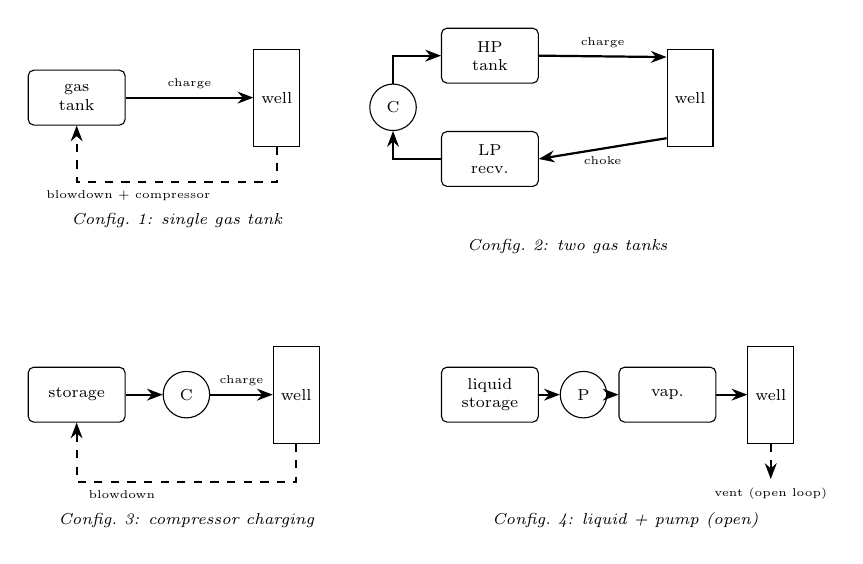
\begin{tikzpicture}[
  scale=0.82, every node/.style={transform shape},
  vessel/.style={draw, rounded corners=2pt, minimum width=1.5cm,
                 minimum height=0.85cm, align=center, font=\scriptsize},
  mach/.style={draw, circle, minimum size=0.72cm, align=center,
               font=\scriptsize, inner sep=1pt},
  well/.style={draw, minimum width=0.5cm, minimum height=1.5cm,
               align=center, font=\scriptsize},
  lbl/.style={font=\scriptsize\itshape},
  flow/.style={-{Stealth[length=2mm]}, thick}]
% Config 1
\begin{scope}
\node[vessel] (t1) at (0,0) {gas\\tank};
\node[well] (w1) at (3.1,0) {well};
\draw[flow] (t1) -- node[above,font=\tiny]{charge} (w1);
\draw[flow, dashed] (w1.south) |- ++(-1.5,-0.55) -| (t1.south)
  node[pos=0.25, below, font=\tiny]{blowdown + compressor};
\node[lbl] at (1.55,-1.9) {Config.\ 1: single gas tank};
\end{scope}
% Config 2
\begin{scope}[xshift=6.4cm]
\node[vessel] (hp) at (0,0.65) {HP\\tank};
\node[vessel] (lp) at (0,-0.95) {LP\\recv.};
\node[well] (w2) at (3.1,0) {well};
\node[mach] (c2) at (-1.5,-0.15) {C};
\draw[flow] (hp.east) -- node[above,font=\tiny]{charge} (w2.120);
\draw[flow] (w2.240) -- node[below,font=\tiny]{choke} (lp.east);
\draw[flow] (lp.west) -| (c2.south);
\draw[flow] (c2.north) |- (hp.west);
\node[lbl] at (1.2,-2.3) {Config.\ 2: two gas tanks};
\end{scope}
% Config 3
\begin{scope}[yshift=-4.6cm]
\node[vessel] (t3) at (0,0) {storage};
\node[mach] (c3) at (1.7,0) {C};
\node[well] (w3) at (3.4,0) {well};
\draw[flow] (t3) -- (c3);
\draw[flow] (c3) -- node[above,font=\tiny]{charge} (w3);
\draw[flow, dashed] (w3.south) |- ++(-2.0,-0.6) -| (t3.south)
  node[pos=0.25, below, font=\tiny]{blowdown};
\node[lbl] at (1.7,-1.95) {Config.\ 3: compressor charging};
\end{scope}
% Config 4
\begin{scope}[xshift=6.4cm, yshift=-4.6cm]
\node[vessel] (t4) at (0,0) {liquid\\storage};
\node[mach] (p4) at (1.45,0) {P};
\node[vessel] (v4) at (2.75,0) {vap.};
\node[well] (w4) at (4.35,0) {well};
\draw[flow] (t4) -- (p4); \draw[flow] (p4) -- (v4);
\draw[flow] (v4) -- (w4);
\draw[flow, dashed] (w4.south) -- ++(0,-0.55)
  node[below, font=\tiny]{vent (open loop)};
\node[lbl] at (2.1,-1.95) {Config.\ 4: liquid + pump (open)};
\end{scope}
\end{tikzpicture}
\caption{Block process-flow sketches of Configurations 1--4
(C = compressor, P = pump; dashed = discharge path). Configuration 5
is \cref{fig:pfd-rec}.}
\label{fig:pfd-configs}
\end{figure}

\begin{figure}[htb]
\centering
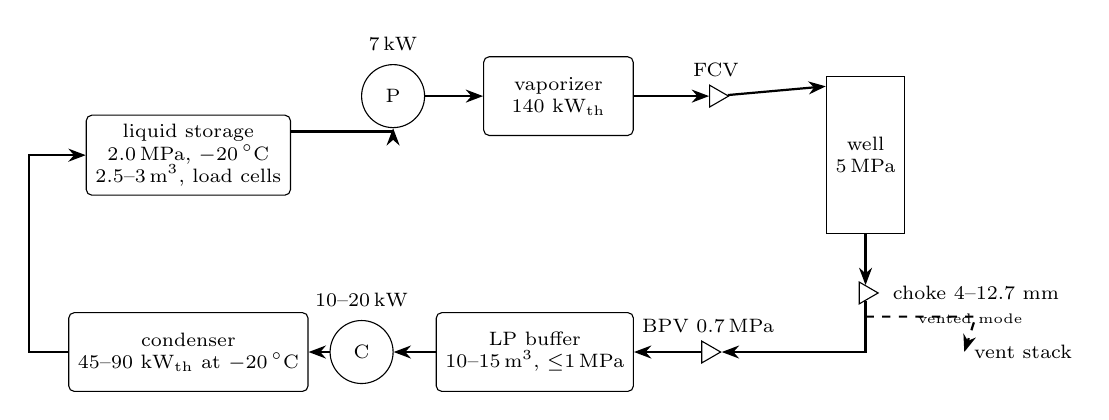
\begin{tikzpicture}[
  vessel/.style={draw, rounded corners=2pt, minimum width=1.9cm,
                 minimum height=1.0cm, align=center, font=\scriptsize},
  mach/.style={draw, circle, minimum size=0.8cm, align=center,
               font=\scriptsize, inner sep=1pt},
  valve/.style={draw, regular polygon, regular polygon sides=3,
                shape border rotate=270, minimum size=0.32cm,
                inner sep=0pt, font=\tiny},
  well/.style={draw, minimum width=0.6cm, minimum height=2.0cm,
               align=center, font=\scriptsize},
  lbl/.style={font=\scriptsize},
  flow/.style={-{Stealth[length=2.2mm]}, thick}]
\node[vessel] (stor) at (0,0)
  {liquid storage\\ \SI{2.0}{MPa}, $-20\,^{\circ}$C\\ 2.5--\SI{3}{m^3}, load cells};
\node[mach] (pump) at (2.6,0.75) {P};
\node[lbl, above=0.05 of pump] {\SI{7}{kW}};
\node[vessel] (vap) at (4.7,0.75) {vaporizer\\ 140 kW$_{\mathrm{th}}$};
\node[valve] (fcv) at (6.7,0.75) {};
\node[lbl, above=0.02 of fcv] {FCV};
\node[well] (well) at (8.6,0) {well\\ \SI{5}{MPa}};
\node[valve] (chk) at (8.6,-1.75) {};
\node[lbl, right=0.05 of chk] {choke 4--12.7 mm};
\node[valve] (bpv) at (6.6,-2.5) {};
\node[lbl, above=0.02 of bpv] {BPV \SI{0.7}{MPa}};
\node[vessel] (buf) at (4.4,-2.5)
  {LP buffer\\ 10--\SI{15}{m^3}, $\le$\SI{1}{MPa}};
\node[mach] (comp) at (2.2,-2.5) {C};
\node[lbl, above=0.05 of comp] {10--\SI{20}{kW}};
\node[vessel] (cond) at (0,-2.5)
  {condenser\\ 45--90 kW$_{\mathrm{th}}$ at $-20\,^{\circ}$C};
\node[lbl] (vent) at (10.6,-2.5) {vent stack};
\draw[flow] (stor.east) ++(0,0.3) -| (pump.south);
\draw[flow] (pump) -- (vap);
\draw[flow] (vap) -- (fcv);
\draw[flow] (fcv) -- (well.120);
\draw[flow] (well.south) -- (chk.north);
\draw[flow] (chk.south) |- (bpv.east);
\draw[flow] (bpv.west) -- (buf.east);
\draw[flow] (buf.west) -- (comp.east);
\draw[flow] (comp.west) -- (cond.east);
\draw[flow] (cond.west) -| ++(-0.5,1.2) |- (stor.west);
\draw[flow, dashed] (chk.south) ++(0,-0.2) -| ++(1.4,0) -- (vent.west)
  node[pos=0.5, above, font=\tiny]{vented mode};
\end{tikzpicture}
\caption{Recommended configuration (5): liquid-anchored closed loop
with a vented reference mode. FCV = flow-control valve, BPV =
back-pressure valve, P = cryogenic pump, C = recovery compressor.
Relief devices, isolation valves, and instrumentation (\S II.9--II.10)
omitted for clarity.}
\label{fig:pfd-rec}
\end{figure}

\section{II.5 Storage: how much, in what phase}

Sizing from the cold-column worst case with margin:
$m_{\mathrm{stor}} = 1.5 \times \SI{2.1}{t} \approx \SI{3.2}{t}$,
i.e.\ a \SI{3}{m^3}-class refrigerated vessel at
\SI{2.0}{MPa}/\SI{-20}{\celsius} --- squarely the commercial CO$_2$
``mini-bulk'' class (3--6 t, factory-insulated, packaged
refrigeration), available for purchase or rental from industrial-gas
suppliers, which is itself a strong argument for this anchor state:
the long-lead, code-stamped component becomes a catalog item. Storage
capacity should be based on \emph{total} inventory (not per-cycle
transfer): the closed loop holds one inventory that migrates between
well and storage, and the 1.5$\times$ factor covers heel, vapor head,
and commissioning losses. The storage pressure band
\SIrange{1.7}{2.3}{MPa} (\SI{-25}{} to \SI{-15}{\celsius}) trades
refrigeration duty against pump suction margin; \SI{2.0}{MPa} is the
conventional center. The minimum information to finalize sizing:
confirmed bore volume per completion string actually used
(\SI{13.9}{m^3} for the 7-5/8\,in string modeled in Part I), the
coldest planned initial condition, and the heel the pump can reach.

\section{II.6 Compressor versus pump: the division of labor}

The intuition that ``a compressor displaces CO$_2$ from one vessel to
another'' conflates three distinct operations with three different
costs. (i) \emph{Pumping liquid}: work
$w \approx v\,\Delta p/\eta$; with
$v = \SI{0.97e-3}{m^3/kg}$, \SIrange{2.0}{6.5}{MPa} and
$\eta = 0.65$, $w = \SI{6.7}{kJ/kg}$ --- \SI{7}{kW} at \SI{1}{kg/s},
discharge temperature essentially unchanged (\SI{-16.5}{\celsius}).
(ii) \emph{Compressing gas}: work scales with
$\int v\,dp$ at gas-phase specific volume, two orders of magnitude
larger; \SIrange{0.7}{2.2}{MPa} costs \SI{101}{kJ/kg}
($\eta_s = 0.70$) and lands at \SI{143}{\celsius}, demanding
aftercooling; ratios above $\sim$4 per stage force multistage
machines with intercooling. (iii) \emph{Pressure-driven transfer}:
free, but consumes the source vessel's state --- the \SI{28}{m^3}
sizing result of \S II.3-A is the price of using a gas vessel's own
pressure as the driver. The division of labor follows: the
\emph{pump} does the high-pressure lift (charging), because the fluid
is liquid there and the lift is cheap; the \emph{compressor} does the
low-pressure gathering (recovery), because the fluid is unavoidably
gas there and the ratio is modest; \emph{passive transfer} is used
only where it is free of state consequences (blowdown itself, and
gravity-fed pump suction). Both machines are justified --- but the
compressor is a \SI{10}{}--\SI{20}{kW} recovery unit, not the
\SI{50}{kW}-class charging machine of the initial concept. Per cycle
(\SI{1563}{kg}): pump 2.9 kWh$_{e}$; vaporizer
124 kWh$_{\mathrm{th}}$ (ambient-air units make most of this free);
recovery compression 44 kWh$_{e}$; condensation
195 kWh$_{\mathrm{th}}$ rejected at \SI{-20}{\celsius}
($\approx$100--130 kWh$_{e}$ at packaged-unit COP 1.5--2).
Liquid pumping beats gas compression for the charging duty by a
factor of $\sim$15 in specific work --- but the honest accounting
shows the cycle's real energy sits in the recovery refrigeration, not
in either machine.

\section{II.7 Equipment sizing methodology}

Governing relations, stated so the numbers above are reproducible and
re-sizable: vessel inventories from
$m = \rho(p,T)\,V$ with Span--Wagner $\rho$; the well inventory from
$m_{\mathrm{well}} = \int_0^L \rho\bigl(p(z),T(z)\bigr)A\,dz$ with
the Part-I hydrostatic--geothermal profile (evaluated numerically by
the model's initializer); pump power $\dot W = \dot m\,\Delta h_s/\eta$
with $\Delta h_s$ along the liquid isentrope; compressor power the
same along the gas isentrope, staged when $p_2/p_1 \gtrsim 4$;
vaporizer and condenser duties as enthalpy differences between the
anchor states; receiver volumes from $V = \Delta m/\rho(p_{\max},T)$;
charging and recovery times from $\Delta m/\dot m$; blowdown duration
from the Part-I model itself (e.g.\ wellhead-pressure half-life
\SI{494}{s} for the 12.7 mm choke at $C_d = 0.84$). Sensitivities
worth carrying into detailed design: all gas-side densities scale
$\sim p/T$, so receiver sizing is robust; the near-critical states
are the opposite (\S II.3-A) and should simply be avoided; vaporizer
duty varies $\pm$15\,\% across the storage band; compressor work is
insensitive to suction temperature but linear in $\ln(p_2/p_1)$.

\section{II.8 Energy and turnaround comparison}

Per full cycle, Configuration 5: $\approx$47 kWh$_{e}$ of machine
work plus 100--130 kWh$_{e}$ of refrigeration --- order
\$20--40 of electricity --- against $\approx$\SI{1.6}{t} of CO$_2$
(order \$300--600 at merchant prices, \emph{[commodity prices
indicative only]}) saved per run relative to venting. The loop pays
for its operating cost in avoided gas after a handful of runs; the
capital trade is the condenser/refrigeration train against the
otherwise-necessary receiver volume, and \S II.1 item 2 settles that
in the condenser's favor by an order of magnitude in vessel size.
Turnaround: charge \SI{\sim 1}{h}, experiment
\SIrange{0.3}{1.2}{h}, recovery \SIrange{2.2}{4.3}{h}
(compressor-limited), thermal soak of the formation to the geothermal
initial state: hours--overnight (conduction-limited, not
equipment-limited). One experiment per day with an overnight soak is
the natural cadence; a second daily run is possible at the cost of a
non-equilibrium (but model-characterizable) initial thermal state.

\section{II.9 Instrumentation and control}

Actively \emph{controlled}: charging mass flow (FCV on Coriolis
feedback), vaporizer outlet superheat ($\ge$\SI{10}{K} above the
injection-line dew point), closed-mode back pressure (BPV setpoint
\SIrange{0.55}{1.0}{MPa}), storage temperature (packaged
refrigeration), compressor suction pressure (recycle/unload).
\emph{Measured}: wellhead and choke-upstream/downstream $p$,$T$ (fast
transducers at the wellhead --- the Part-I wave analysis implies
$\gtrsim$\SI{100}{Hz} to resolve the expansion-wave arrival and
reflections); Coriolis mass flow on the charge line; blowdown mass
flow \emph{by inference} --- choke-model + upstream state, closed by
storage-vessel load cells and buffer $p$,$T$ inventory accounting ---
because a Coriolis meter in the discharge line would see flashing
two-phase flow, where its reading is not trustworthy; the existing
completion DTS for distributed temperature (the Part-I/Part-II
saturation-thermometer opportunity); tank levels by differential
pressure plus load cells; O$_2$/CO$_2$ area monitors. The control
philosophy mirrors the model architecture deliberately: every
controlled boundary of the facility (charge flow, back pressure,
storage state) is an input the Part-I model already accepts, which is
what makes the digital-twin coupling of \S II.11 a bookkeeping
exercise rather than a re-formulation.

\section{II.10 Safety (conceptual; formal review required)}

The hazards are the standard dense-CO$_2$ set, concentrated as
follows. \emph{Trapped-liquid overpressure}: any liquid-full segment
between two valves (pump discharge line, condensate return) generates
extreme pressure on warming; every such segment needs a thermal
relief valve --- this is the single most common CO$_2$-facility
design error. \emph{Two-phase/flashing relief}: relief devices on
liquid or dense service must be sized by HEM/omega-method two-phase
methods (API 520 Annex C; ISO 4126-10), not gas formulas --- the same
physics as the Part-I choke analysis, and \citet{hammer2022} shows
HEM sizing errs conservative (low) on flow, which for relief sizing
is the \emph{non}-conservative direction; a margin policy is
required. \emph{Dry ice}: vent and relief paths cross the triple
pressure by design; they must be short, straight, downward-sloping,
single-walled where blockage matters, and rated for
\SI{-78}{\celsius} impingement (low-temperature-toughness material
selection per B31.3); the closed-mode BPV floor of \SI{0.55}{MPa} is
itself a dry-ice control. \emph{Asphyxiation}: a full inventory
release is \SI{\sim 1.6}{t} of CO$_2$; outdoor, elevated vent
discharge, area monitors with alarm-at-\SI{0.5}{\%}/evacuate
levels, and attention to low-lying accumulation (CO$_2$ is
1.5$\times$ air density). \emph{Machine protection}: compressor
suction knockout (liquid carryover from the buffer on cold days),
pump minimum-flow recycle, high-discharge-temperature trips.
\emph{Codes}: ASME BPVC VIII vessels, B31.3 process piping, API
520/521 relief, with CGA/EIGA CO$_2$-specific guidance
\emph{[standard designations to be confirmed in formal review]}.
Pressure ratings: the charging side sees \SI{6.5}{MPa} + relief
margin; the well and wellhead govern themselves under existing
facility certification.

\section{II.11 Coupling to the wellbore model: the digital twin}

The surface equipment is lumped-parameter by construction --- every
vessel is a well-mixed mass/energy accumulator,
\begin{equation}
\frac{dM_i}{dt} = \sum_j \dot m_{ij},
\qquad
\frac{d(M_i u_i)}{dt} = \sum_j \dot m_{ij} h_{ij}
 + \dot Q_i + \dot W_i,
\label{eq:lumped}
\end{equation}
closed by Span--Wagner $(\rho, u) \to (p, T, x)$ --- the \emph{same}
UV-flash primitive recovery as the Part-I two-phase wellbore closure,
so one thermodynamic kernel serves the entire twin. Valves and chokes
use the Part-I HEM orifice flux (already implemented); the
charging FCV is the identical model run in reverse service; the
compressor is a map $\dot m(p_s, p_d, N)$ with isentropic efficiency;
the pump is $\dot m$-prescribed with \cref{eq:lumped} bookkeeping;
heat exchangers are effectiveness--NTU duties. Connecting piping
(tens of meters) has negligible volume next to the well
(\SI{13.9}{m^3}) and buffer; it needs distributed treatment only if
surface-line acoustics themselves become a measurement target. The
coupling to the distributed wellbore model is through exactly one
interface --- the wellhead boundary condition --- and the Part-I
choke closure already takes the downstream pressure as a parameter:
replacing the constant $p_b$ with the buffer state
$p_b = p_{\mathrm{buf}}(t)$ from \cref{eq:lumped}, integrated
explicitly at the wellbore time step (the buffer's fill time of
minutes against acoustic steps of milliseconds makes the explicit
coupling error negligible, by the same time-scale argument as the
Part-I conjugate thermal coupling), turns the existing solver into
the discharge half of the twin with no structural change. Mass and
energy conservation across the facility then reduces to summing
\cref{eq:lumped} over vessels plus the wellbore budgets the Part-I
code already closes to machine precision --- giving the twin a
built-in, auditable conservation check, and giving leak detection a
quantitative baseline.

\section{II.12 Recommendation}

\textbf{A. One tank or two?} Two vessels, but not the two of the
initial concept: one refrigerated \emph{liquid} storage
(3 t class) as the reproducible anchor, plus one modest LP gas
\emph{buffer} (10--\SI{15}{m^3}) as shock absorber --- not a second
full-inventory gas tank.
\textbf{B. Compressor for charging?} No. Charging is pump +
vaporizer; passive transfer alone also fails (\S II.3-A). The
compressor belongs on recovery, at one-fifth the power the charging
duty would demand of it.
\textbf{C. Liquid pump advantages?} Decisive: \SI{6.7}{} vs
\SI{101}{kJ/kg}, \SI{7}{kW} vs tens of kW, no discharge-temperature
management, catalog cryogenic hardware. Its obligations ---
flooded suction, NPSH, thermal-relief of liquid-full segments --- are
standard practice.
\textbf{D. Storage phase?} Saturated liquid at
\SI{2.0}{MPa}/\SI{-20}{\celsius}. Gas storage fails on volume,
ambient-temperature liquid on the critical point and
thermal-expansion hazard, near-critical dense fluid on
reproducibility.
\textbf{E. LP receiver rather than direct return?} Yes ---
structurally necessary, since the blowndown stream can neither enter
the \SI{2}{MPa} storage unaided nor be condensed at its instantaneous
peak rate; the buffer decouples the fast experiment from the slow
recovery train.
\textbf{F. Reset procedure?} Compressor--condenser transfer at
\SIrange{0.1}{0.2}{kg/s} (\SIrange{2.2}{4.3}{h}), concurrent with an
overnight formation soak for geothermal initial conditions.
\textbf{G/H. Best configuration, and easiest to model?} The same one
--- Configuration 5 --- and not coincidentally: its control variables
are exactly the model's boundary conditions (\S II.9, \S II.11).
\Cref{tab:matrix} summarizes.

\begin{table}[htb]
\centering
\small
\caption{Configuration comparison. ++ favorable, $-$ unfavorable,
$\circ$ neutral/conditional. Capital and operating costs are
order-of-magnitude judgments at concept level.}
\label{tab:matrix}
\begin{tabular}{lccccc}
\toprule
Criterion & C1 single & C2 two-gas & C3 compr. & C4 liq.\ open &
C5 hybrid \\
\midrule
Capital cost & $\circ$ & $-$ & $\circ$ & ++ & $\circ$ \\
Operating cost/energy & $-$ & $-$ & $-$ & $\circ$ & + \\
Equipment complexity & + & $-$ & $\circ$ & ++ & $\circ$ \\
Operational flexibility & $-$ & $\circ$ & $-$ & $\circ$ & ++ \\
Repeatability of ICs & $-$ & $-$ & $\circ$ & ++ & ++ \\
CO$_2$ retention (closed) & $\circ$ & + & $\circ$ & $-$ & ++ \\
Vessel volumes & $-$ & $-$ & + & ++ & + \\
Safety profile & $\circ$ & $\circ$ & $\circ$ & + & + \\
Ease of control & $-$ & $-$ & $-$ & + & + \\
Digital-twin suitability & $\circ$ & $\circ$ & $-$ & + & ++ \\
Future research headroom & $-$ & $\circ$ & $-$ & $\circ$ & ++ \\
\bottomrule
\end{tabular}
\end{table}

\paragraph{Development strategy.} \emph{Phase 1 (essential, enables
first experiments)}: liquid storage vessel, pump, vaporizer, charging
FCV + Coriolis, vent stack, wellhead fast instrumentation, relief and
gas-detection systems --- this is Configuration 4 and runs vented
reference blowdowns that validate the Part-I/Part-II models.
\emph{Phase 2 (closes the loop)}: LP buffer, BPV, recovery
compressor, condenser, load-cell inventory accounting --- converts
the same facility to Configuration 5 without rework, enabling
repeated closed-cycle campaigns and the reduced-choke experiments.
\emph{Optional/later}: second completion-string tie-ins, a
surface test section for choke-model experiments
(\citealp{hammer2022} geometry), slipstream impurity dosing.

\paragraph{Unresolved before detailed engineering.} Confirmed
completion string(s) and wellhead rating for repeated thermal
cycling; coldest intended initial condition (sets storage margin and
materials); site power available for the refrigeration train;
acceptable per-run venting policy (regulatory and institutional);
relief-study basis (full-bore charging-line failure vs choke stuck
open); merchant CO$_2$ supply logistics for first fill and makeup;
and the choke-hardware plan (fixed beans vs adjustable), which fixes
whether $C_d$ calibration (Part I, \S 10) happens on the well or on a
surface test section.

\section{II.13 References and precedents for the facility concept}

The closed-loop architecture has direct precedents in the
depressurization rigs reviewed in Part I: the SINTEF ECCSEL
depressurization facility \citep{munkejord2020, munkejord2021}
(instrumentation density and data practices worth copying: 100 kHz
pressure arrays, triplet thermocouples, open raw data), the
\citet{hammer2022} orifice test section (the natural template for a
surface choke-calibration leg), and the large-scale vented programs
(COOLTRANS; \citealp{cosham2012}) whose venting practice ---
vertical stacks, dry-ice-tolerant design --- informs the vented mode.
No published facility performs repeated \emph{wellbore-scale}
closed-loop CO$_2$ charge/discharge cycles; that is the same
experimental gap identified in Part I (\S 14H), and this facility is,
to the knowledge assembled here, the instrument that would fill it.


\bibliographystyle{plainnat}
\bibliography{references}

\end{document}
